\documentclass[pt, qual, classic, oneside, a4paper, scr]{ufba/ufbathesis}


\usepackage[utf8]{inputenc}
%\usepackage[ansinew]{inputenc}
\usepackage{graphicx}
\usepackage{lipsum}
\usepackage{hyphenat}
\usepackage[usenames, dvipsnames, table]{xcolor}
\usepackage{booktabs}
\usepackage{pifont}
\usepackage{multicol}
\usepackage{multirow}
\usepackage{listings} 
\usepackage{colortbl}
\usepackage{xfrac}
\usepackage[FIGTOPCAP]{subfigure}
\usepackage[printonlyused, withpage]{acronym}
\usepackage{enumitem}
\usepackage{longtable}
\usepackage{lscape}
\usepackage{todonotes}
\usepackage{mathtools}



\university{Universidade Federal da Bahia}
\address{Salvador}
\institute{Instituto de Matem\'{a}tica e Estatística}
\library{Biblioteca Reitor Macedo Costa}
\program{Programa de Pós-Graduação em Ciência da Computação}
\majorfield{Ciência da Computação}
\title{AVALIAÇÃO EMPÍRICA DA APLICAÇÃO DAS TÉCNICAS DE SELEÇÃO DE TESTE DE REGRESSÃO IMPLEMENTADAS POR FERRAMENTAS EM APLICAÇÕES ANDROID}
\date{Agosto/2020}
\defenseyear{2020}
\author{Sara Mendes Oliveira Lima}
\adviser{Prof. Dr. Ivan do Carmo Machado}
\coadviser{Dra. Larissa Rocha Soares}

\begin{document}
\pgcompfrontpage
\frontmatter

\pgcomppresentationpage

%%%%%%%%%%%%%%%%%%%%%
% Resumo em Portugues
%%%%%%%%%%%%%%%%%%%%%

\resumo


No desenvolvimento de software, a garantia da qualidade é um fator de grande importância. O teste de software é uma das estratégias que pode ser utilizada. Com o processo constante de evolução de software, orientado pelas manutenções realizadas, para garantir que as mudanças realizadas não alterem o comportamento do sistema faz-se uso do Teste de Regressão. Testes de regressão apresentam-se como uma estratégia viável para lidar com a complexidade, e com a constante evolução, dos sistemas de software, incluindo os \ac{APPS}, que tem sido cada vez mais utilizados no cotidiano. Embora a literatura tenha dedicado esforços à produzir evidências sobre a criação de novas técnicas de teste de regressão para Android,  o sistema operacional mais popular para os dispositivos móveis, os estudos existentes são bastante limitados no que diz respeito a demonstrar evidências empíricas que garantam quais são as técnicas implementadas por ferramentas mais aplicáveis no desenvolvimento de \ac{APPS} Android. Neste contexto, este estudo tem como objetivo realizar uma avaliação empírica das técnicas de seleção de teste de regressão implementadas por ferramentas aplicadas a \ac{APPS} Android. Para tanto, a pesquisa foi organizada em quatro etapas: etapa conceitual; realização de uma revisão estruturada da literatura sobre técnicas de teste de regressão para \ac{APPS} Android; aplicação de um \textit{Survey} e de entrevistas, para compreensão de como estudantes / profissionais realizam teste de regressão; e realização de um estudo experimental sobre técnicas de teste de regressão implementadas por ferramentas para \ac{APPS} Android. Ao final da pesquisa, espera-se as seguintes contribuições: corpo de conhecimento sobre o uso de técnicas de teste de regressão para o desenvolvimento de \ac {APPS} Android; prover evidências empíricas sobre quais as técnicas de teste de regressão implementadas por ferramentas são mais adequadas para projetos de \ac{APPS} Android; identificar como a indústria realiza o teste de regressão em \ac{APPS} Android; e apresentar ferramentas de teste de regressão disponíveis para projetos Android.



% Palavras-chave do resumo em Portugues
\begin{keywords}
Evolução de Software; Qualidade de Software; Teste de Regressão; APPS Android; Ferramentas.
\end{keywords}

%%%%%%%%%%%%%%%%%%%
% Resumo em Ingles
%%%%%%%%%%%%%%%%%%%



\abstract


%\textit{
In software development, quality assurance is a major factor. Software testing is one of the strategies that can be used. With the constant process of software evolution, guided by the maintenance performed, to ensure that the changes made do not alter the system behavior, the Regression Test is used. Regression testing is a viable strategy for dealing with the complexity and constantly evolving software systems, including APPS, which has been increasingly used in everyday life. While the literature has devoted efforts to produce evidence on the creation of new regression testing techniques for Android, the most popular mobile operating system, existing studies are quite limited in demonstrating empirical evidence to ensure which ones are. the techniques implemented by most applicable tools in Android \ac {APPS} development. In this context, this study aims to perform an empirical evaluation of regression testing techniques implemented by Android \ac {APPS} tools. To this end, the research was organized in four stages: conceptual stage; conducting a systematic mapping of regression testing techniques for \ac {APPS} Android; applying a Survey and interviews, to understand how students / professionals perform regression testing; and conducting an experimental study on regression testing techniques implemented by tools for \ac {APPS} Android. At the end of the research, the following contributions are expected: body of knowledge on the use of regression testing techniques for the development of Android \ac {APPS}; provide empirical evidence on which tool-implemented regression testing techniques are best suited for Android \ac {APPS} projects; identify how industry conducts regression testing on \ac {APPS} Android; and present regression testing tools available for Android projects.
%}.

% Palavras-chave do resumo em Ingles
\begin{keywords}
%\textit{
Software Evolution; Software quality; Regression Testing; APPS Android; Tools.%}.
\end{keywords}

\tableofcontents
\listoffigures
\listoftables

\chapter*{Lista de Siglas}

\begin{acronym}[PGCOMP]
    \acro{APPS}{Aplicativos para Dispositivos Móveis}
    \acro{QA}{\textit{Quality Assurance}}
    \acro{GQM}{\textit{Goal-Question-Metric Approach}}
    \acro{OTAN}{{Organização do Tratado do Atlântico Norte}}
    \acro{RTS}{\textit{Regression Test Case Selection}}
    \acro{SQA}{\textit{Software Quality Assurance}}
    \acro{SUT}{\textit{System Under Test}}
    \acro{VV}{Verificação e Validação}
\end{acronym}

\mainmatter

\xchapter{Introdução}{}

\acresetall 


Este capítulo apresenta o contexto em que a presente investigação se insere, enfatizando: a apresentação; o problema; os objetivos; as questões de pesquisa; a metodologia; os resultados esperados e como o trabalho está estruturado.

\section{Apresentação}\label{sec:apresentacao}
Desenvolver software não é uma tarefa simples e envolve diversas condicionais, tais como: escopo, prazo e recursos disponíveis. Nesse processo, um problema que pode ocorrer é entregar algo diferente do que era esperado pelo cliente. Isso acontece na maioria das vezes porque as atividades de desenvolvimento dependem da capacidade de interpretação e execução das pessoas que as constroem. Para que esses erros não perdurem e para que se possa identificá-los antes de liberar o software para utilização, existe uma série de atividades, coletivamente chamadas de Validação, Verificação e Teste \cite{DELAMARO2007}. 

\ac{VV} permite que se determine sistematicamente se os requisitos de um sistema estão sendo corretamente tratados e implementados. A atividade de testes tem por objetivo descobrir defeitos no software, considerando aspectos estruturais e lógicos. Verificar, validar e testar software auxiliam na Garantia de Qualidade do mesmo. Garantia de Qualidade, do termo comumente utilizado (em inglês) \ac{QA}, é o processo geral de definição de como a qualidade de software pode ser alcançada, e como a organização de desenvolvimento sabe que o software tem o nível de qualidade necessário. \ac{QA} estabelece processos, procedimentos e padrões que conduzem a um software de qualidade \cite{HIRAMA2011}. 

O presente trabalho tem como foco a atividade de teste. Os testes são normalmente executados e reportados durante as etapas de desenvolvimento do software. Espera-se que haja uma grande massa de testes realizada antes de se disponibilizar uma versão estável do software. Entretanto, existe uma técnica de testes, denominada \textbf{teste de regressão}, que deve ser considerada quando é necessário realizar a manutenção do software, quer perfectiva, corretiva, adaptativa ou preventiva \cite{DBLP:series/springer/Mens08}. O teste de regressão tem como objetivo fornecer confiança de que as alterações recém-introduzidas não obstruem os comportamentos da parte existente e inalterada do software \cite{Yoo:2012:RTM:2284811.2284813}.

No teste de regressão, há a reexecução de todos os casos de testes da versão original do software. Esse procedimento tende a gerar um grande esforço da equipe de testes, a depender da quantidade de casos de teste. A literatura apresenta uma série de técnicas para lidar com este problema, em particular no sentido de propor mecanismos para reduzir o número de reexecuções de casos de testes, sem perder a cobertura do código fonte e a capacidade de detecção de falhas ,\cite{65194}, \cite{WHITE1991}, \cite{Graves:2001:ESR:367008.367020}, \cite{630875}, \cite{536955}, \cite{ENGSTROM201014},\cite{ENGSTROM201014}, \cite{KAZMI2017}, \cite{ROMANO201862}. Segundo \citeonline{Yoo:2012:RTM:2284811.2284813} as técnicas de Teste de Regressão são classificadas como: Técnicas de Seleção; Técnicas de Minimização; e Técnicas de Priorização.  

Dentre os domínios de aplicação emergentes, testes de regressão apresentam-se como uma estratégia viável para lidar com a complexidade - e a constante evolução - dos \ac{APPS}. Neste cenário, o presente trabalho tem como foco a análise da evolução das técnicas de seleção de teste de regressão no desenvolvimento de \ac{APPS} para Android.


\section{Problema}\label{sec:problema}

Os dispositivos móveis tem sido cada vez mais utilizados no cotidiano, em alguns casos com maior parcela de mercado do que os tradicionais Desktop \cite{Do2016RedroidAR}. Pesquisas de mercado recentes indicam que o \textbf{Android} é o sistema operacional mais popular para os dispositivos móveis - vide Figura \ref{fig:marketShare}\footnote{\url{http://gs.statcounter.com/os-market-share/mobile/worldwide}}. 

Segundo \citeonline{Do2016RedroidAR}, a plataforma móvel está se separando de uma variedade de áreas de aplicativos de Desktop, tais como entretenimento, comércio eletrônico e mídia social. Assim, os desenvolvedores são obrigados a produzir \ac{APPS} de alta qualidade, em particular no que diz respeito a requisitos não-funcionais como portabilidade, confiabilidade e segurança.


\begin{figure}
    \centering
    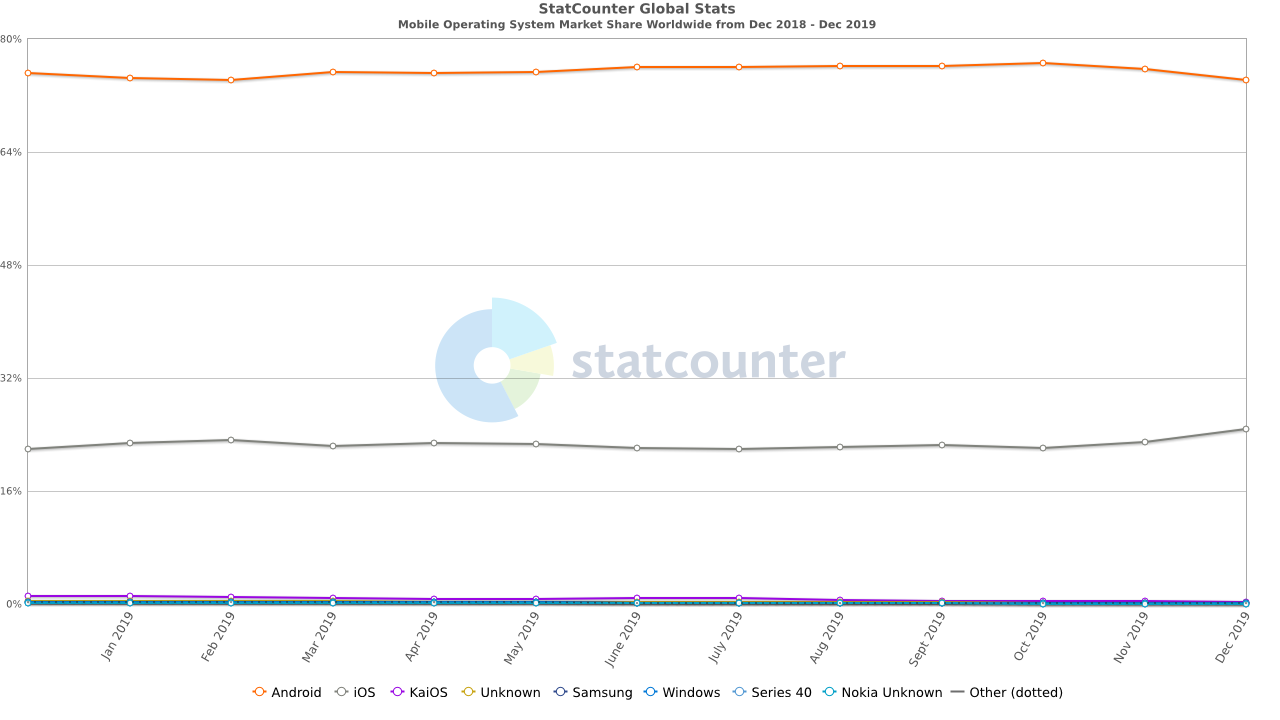
\includegraphics[width=1.\textwidth]{images/StatCounter-os_2020.png}
    \caption{Distribuição mundial do uso de sistemas operacionais para \ac{APPS}.}
    \label{fig:marketShare}
\end{figure}


Nos últimos anos, uma grande quantidade de pesquisas tem sido realizada para prover uma maior confiabilidade dos \ac{APPS}, por exemplo, aplicando testes automatizados \cite{7927972}, \cite{8424973},\cite{8453877}. No entanto, a maioria das pesquisas está focada no teste de uma versão única de aplicativos móveis \cite{Do2016RedroidAR}. Como os \ac{APPS} evoluem com frequência, é importante que os desenvolvedores façam uso de técnicas de teste de regressão, dado seu potencial em identificar problemas no código decorrentes de mudanças no software \cite{8377661}.


Ao tratar de técnicas de teste de regressão, a literatura apresenta diversos trabalhos que fazem uso de técnicas tradicionais, i.e., concebidas para testar sistemas Desktop \cite{536955}, \cite{ENGSTROM201014}. Entretanto, embora muitas abordagens eficientes e eficazes tem sido propostas, há pouca evidência indicando a aplicação direta dessas técnicas para o teste de \ac{APPS} \cite{Do2016RedroidAR}. Um importante fator que causa a incompatibilidade é a diferença entre a arquitetura do sistema da plataforma móvel e a plataforma Desktop.

Segundo \citeonline{5954416}, a qualidade dos \ac{APPS} é geralmente ruim. Um dos fatores da falta de qualidade são processos de desenvolvimento muito rápidos em que a atividade de teste é negligenciada ou conduzida de forma superficial, uma vez que é considerada demasiado complexa, difícil de automatizar, dispendiosa e demorada. 

Em virtude do crescimento do mercado de dispositivos móveis e da necessidade de produzir \ac{APPS} com qualidade, pesquisas recentes tem apresentado o desenvolvimento de técnicas implementadas por ferramentas de teste de regressão voltadas para aplicações em Android \cite{Do2016RedroidAR}, \cite{Choi:2018:DMA:3180155.3180173}, \cite{8377661}, \cite{5954416}, \cite{7927972}, \cite{8424973}, \cite{6339502}, \cite{6569773}, \cite{7427895}, \cite{7832883}, \cite{7833000}. Alguns desses estudos tratam de experimentos com comprovação empírica para comprovar a eficiência/eficácia da ferramenta proposta neste cenário.

Embora a literatura tenha dedicado esforços à produzir evidências sobre a criação de novas técnicas de teste de regressão para Android, os estudos existentes são bastante limitados no que diz respeito a demonstrar evidências empíricas que garantam quais são as técnicas de seleção de teste de regressão implementadas por ferramentas mais aplicáveis no desenvolvimento de \ac{APPS} Android. Neste sentido, é fundamental que novas pesquisas sejam desenvolvidas, de modo a ampliar o conjunto de evidências sobre essa aplicabilidade. 

Dado a complexidade do problema ora descrito, este estudo buscará responder à seguinte questão de pesquisa principal:
\leavevspace 

\begin{center}
    \noindent\fbox{ 
        \parbox{.8\textwidth}
        {
        \begin{center}
            
            \textbf{Quais são as técnicas de seleção de teste de regressão implementadas por ferramentas adequadas para projetos de \ac{APPS} Android?}
        \end{center}
        }
    }
\end{center}

\vspace{.5em}

Esta questão foi refinada em questões específicas:
\vspace{.5em}

\begin{enumerate}[label=\bf QP\arabic*,leftmargin=1.8cm]
    
    \item \textbf{Quais são as técnicas de seleção de teste de regressão apresentadas na literatura?} Essa questão de pesquisa será respondida com a revisão estruturada da literatura sobre Técnicas de Seleção de Teste de Regressão.
    
    \item \textbf{Existem ferramentas de teste de regressão aplicadas a \ac{APPS} Android disponíveis para utilização (open source ou proprietárias) implementadas a partir de técnicas de seleção de teste de regressão?} Essa questão de pesquisa será respondida com a revisão estruturada da literatura sobre ferramentas de teste de regressão.
    
    \item \textbf{Qual a perspectiva de acadêmicos e profissionais sobre técnicas de seleção de teste de regressão para projetos de \ac{APPS} Android?} Essa questão de pesquisa será respondida com a aplicação de um \textit{Survey} e realização de estudo experimental.

\end{enumerate}



\subsection{Objetivos}

Compreendendo que o estudo das técnicas de seleção de teste de regressão para Android é um campo em expansão, o presente trabalho tem como objetivo \textbf{realizar uma avaliação empírica das técnicas de seleção de teste de regressão implementadas por ferramentas aplicadas a \ac{APPS} Android.}

Os seguintes objetivos específicos foram definidos para esta investigação:

\begin{enumerate}[label=\bf O\arabic*,leftmargin=1.5cm]

    \item \textbf{Levantar quais são as técnicas de seleção de teste de regressão que a literatura apresenta.} Para alcançar esse objetivo, será realizado uma revisão estruturada de literatura sobre técnicas de seleção de teste de regressão.
    
    \item \textbf{Verificar quais são as ferramentas de teste de regressão aplicadas a \ac{APPS} Android disponíveis para uso (open source ou proprietárias), e se as mesmas foram implementadas baseadas nas técnicas de seleção de teste de regressão.} Para alcançar esse objetivo, será realizado uma revisão estruturada de literatura sobre ferramentas de teste de regressão.
    
    \item \textbf{Identificar como é realizado o processo de teste de software por acadêmicos e profissionais que desenvolvem \ac{APPS} Android.} Para alcançar esse objetivo, será aplicado um \textit{Survey} e realizado experimentos com acadêmicos e profissionais que trabalham com projetos de \ac{APPS} para Android.


\end{enumerate}



\section{Metodologia}\label{sec:metodologia}


Esta Seção apresenta a metodologia utilizada para desenvolver este trabalho e alcançar os objetivos propostos:


\begin{itemize}
  \item \textbf{Fase 1}: Etapa conceitual que tem como objetivo tratar dos conhecimentos referentes ao tema proposto.
  
  
  Esta etapa visa levantar a bibliografia das áreas sob investigação, para compreender conceitos fundamentais. São elas: evolução de software; qualidade de software; testes de software; teste de regressão; e, estratégias de testes de aplicações para dispositivos móveis.
  
  O levantamento bibliográfico foi feito de forma estruturada, com a leitura de livros e artigos sobre os tópicos abordados na pesquisa. Inicialmente uma leitura mais ampla em busca de um conhecimento inicial, e em uma segunda fase, com leituras específicas de textos com relação direta a este trabalho.
  
  \item \textbf{Fase 2}: Refere-se ao Survey.
  
  Esta etapa contempla a aplicação de um Survey para acadêmicos e profissionais que trabalham com \ac{APPS} Android, para compreender como é realizado o processo de teste de \ac{APPS} Android. O Survey foi planejado com base em \cite{Kitchenham:2002:PSR:566493.566495}.
  
  \item \textbf{Fase 3}: Refere-se ao Estudo Experimental.
  
  Esta etapa contempla a execução de experimentos cujo objetivo principal é compreender como as ferramentas disponíveis para testes de \ac{APPS} Android podem auxiliar acadêmicos e profissionais no processo de teste de regressão dos seus aplicativos. O estudo experimental será planejado com base em \cite{Wohlin:2012:ESE:2349018}.
  
\end{itemize}

\section{Resultados Esperados}\label{sec:resultadosesperados}

Ao final deste trabalho, espera-se contribuir com os seguintes resultados:

%Refinar este tópico

\begin{itemize}

    \item Contribuir com o corpo de conhecimento sobre o uso de técnicas de seleção teste de regressão para o desenvolvimento de \ac{APPS} Android, com base na síntese de evidências disponíveis na literatura.
    
    \item Coletar e analisar dados, no sentido de prover evidências empíricas sobre quais as técnicas de seleção de teste de regressão implementadas por ferramentas são mais adequadas para projetos de \ac{APPS} Android.
    
    \item Identificar como a indústria de \ac{APPS} Android realiza teste de regressão.
    
    \item Apresentar o potencial, em termos de \textit{features} implementadas, das ferramentas de teste de regressão disponíveis para projetos Android, e levantar oportunidades para implementações futuras.

\end{itemize}


\section{Estrutura do Trabalho}\label{sec:estruturadotrabalho}

Os demais capítulos desta qualificação estão estruturados como segue: 
\begin{itemize}
\item \textbf{Capítulo 2}: Fundamentação Teórica;
\item \textbf{Capítulo 3}: Técnicas de seleção de teste de regressão;
\item \textbf{Capítulo 4}: Ferramentas de teste de regressão para \ac{APPS} Android;
\item \textbf{Capítulo 5}: \textit{Survey};
\item \textbf{Capítulo 6}: Considerações Finais.
\end{itemize}
\xchapter{Referencial Teórico, Conceitos e Aplicabilidade}{}
\acresetall 
O presente capítulo apresenta os conceitos fundamentais necessários para a compreensão do trabalho proposto: evolução de software; qualidade de software; teste de software; teste de regressão, e técnicas de seleção de teste de regressão.

\section{Evolução de Software}\label{sec:evolucaodesoftware}

%Em 1967, havia uma consciência do crescimento rápido do mercado de desenvolvimento de software, bem como do impacto e da importância da utilização dos mesmos. Além disso, com os diversos problemas enfrentados na fabricação de software, observou-se a necessidade de desenvolvimento de técnicas baseadas em fundamentos teóricos e disciplinas práticas estabelecidas nos ramos tradicionais da engenharia. Esses fatores levaram a realização da primeira conferência sobre Engenharia de Software em 1968. O objetivo desta conferência, organizada pelo Comitê de Ciência da \ac{OTAN}, foi “o estabelecimento e uso de princípios de engenharia para obter software confiável, eficiente e economicamente viável” \cite{DBLP:series/springer/Mens08}.%

O desenvolvimento de um software não termina com a entrega do sistema, mas, refere-se a um processo contínuo durante toda a sua vida útil. Após a entrega e/ou implantação do sistema,%Depois que um sistema é implantado,%
para que ele se mantenha útil, faz-se necessário o processo de evolução do software. A \textbf{evolução} é a fase em que as mudanças significativas na arquitetura e nas funcionalidades do software podem ser feitas. Quando em serviço, as mudanças feitas são relativamente pequenas, essenciais. No processo de evolução, ao decorrer da utilização do software, surgem novas solicitações de mudança, gerando assim novas \textit{releases} do sistema.

Uma das consequências da evolução de um software é a constante necessidade de realizar sua manutenção. A Norma IEEE 1219 \cite{257623} define manutenção de software como a modificação de um produto de software após a entrega para corrigir falhas; melhorar o desempenho ou outros atributos; ou adaptar o produto a uma modificação. \citeonline{DBLP:series/springer/Mens08} classifica o processo de manutenção como: perfectiva, corretiva, adaptativa ou preventiva:

\begin{itemize}
   
    \item \textbf{Manutenção perfectiva}: É qualquer modificação de um produto de software após a entrega com o objetivo de melhorar o desempenho ou a capacidade de manutenção.
   
    \item \textbf{Manutenção corretiva}: Diz respeito às modificações reativas de um produto de software executadas após a entrega para corrigir falhas descobertas.
   
    \item \textbf{Manutenção adaptativa}: É a modificação de um produto de software executada após a entrega para manter um programa de computador utilizável em um ambiente modificado ou em mudança.
   
    \item \textbf{Manutenção preventiva}: Refere-se a modificações de software realizadas com o objetivo de prevenir problemas antes que eles ocorram.

\end{itemize}


\section{Qualidade de Software}\label{sec:qualidadedesoftware}


O termo qualidade é apresentado com diferentes conceitos na literatura. A ISO 9000 define qualidade como o grau
em que um conjunto de características inerentes preenchem os requisitos \cite{iso9000}. Para \citeonline{juran1970quality} e \citeonline {crosby1979quality}, o conceito de qualidade está relacionado à ``conformidade com requisitos'' e ``adequação para
uso'', respectivamente. Para \citeonline{HIRAMA2011}, qualidade é algo difícil de ser definido. Ainda mais difícil é garantir a qualidade de algum produto, visto que a percepção de qualidade passa pelas expectativas que cada pessoa tem sobre algum produto ou serviço. %A resposta do que é qualidade baseia-se nas expectativas dos \textit{stakeholders}, vide Figura \ref{figure:conceitoqualidade}.%


\begin{comment}
\begin{figure}[!htb]
\centering
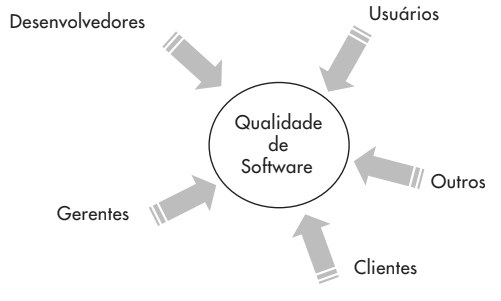
\includegraphics[width=.5\textwidth]{images/conceitoqualidade.png}
\caption{\textit{Stakeholders} e suas expectativas sobre qualidade de software  \cite{HIRAMA2011}}
\label{figure:conceitoqualidade}
\end{figure}
\end{comment}


Tendo em vista a importância da qualidade no processo de desenvolvimento de um software, garantir a qualidade é uma tarefa relevante. Segundo \citeonline{HIRAMA2011}, Garantia de Qualidade, do inglês \ac{QA}, é o processo geral de definição de como a qualidade de software pode ser atingida e como a organização de desenvolvimento sabe que o software tem o nível de qualidade necessário. A garantia de qualidade estabelece processos, procedimentos e padrões que conduzem a um software de qualidade. 

De acordo com \citeonline{HIRAMA2011}, a qualidade de um software está intimamente relacionada à quantidade de defeitos descobertos. Quanto mais defeitos são descobertos, maior é a qualidade do software. %A Figura \ref{figure:ETESTE} ilustra a relação entre qualidade de software e extensão de teste.%

\begin{comment}
\begin{figure}[!htb]
\centering
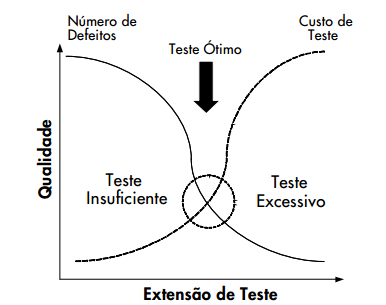
\includegraphics[width=.5\textwidth]{images/ETESTE.png}
\caption{Relação entre qualidade de software e extensão de teste \cite{HIRAMA2011}.}
\label{figure:ETESTE}
\end{figure}
\end{comment}

A próxima seção apresenta os conceitos fundamentais sobre teste de software.


\section{Teste de Software}\label{sec:testesdesoftware}

\subsection{Validação, Verificação e Teste}

Desenvolver software não é uma tarefa simples e envolve diversas condicionais, tais como: escopo, prazo e recurso disponível. Nesse processo, um problema que pode ocorrer é entregar algo diferente do que era esperado pelo cliente. Isso acontece na maioria das vezes por causa de erros humanos, ou seja, porque as atividades de desenvolvimento dependem da capacidade de interpretação e execução das pessoas que as constroem. Para que esses erros não perdurem e para que se possa identificá-los antes de liberar o software para utilização, existe uma série de atividades, coletivamente chamadas de Validação, Verificação e Teste. Em geral, dividem-se as atividades de Validação, Verificação e Teste em estáticas e dinâmicas. As estáticas são as que não requerem a execução ou mesmo a existência de um programa ou modelo executável para serem conduzidas. As dinâmicas são as que se baseiam na execução de um programa ou de um modelo \cite{DELAMARO2007}.

\ac{VV} permite que se determine sistematicamente se os requisitos de um sistema estão sendo corretamente tratados e implementados. A atividade de testes tem por objetivo descobrir defeitos no software, considerando aspectos estruturais e lógicos do software. \ac{VV} contribuem diretamente para o atendimento dos prazos e custos do projeto. Portanto, conhecer os conceitos de \ac{VV} é importante para obter produtos de maior qualidade e produtividade e melhorar os processos continuamente. As atividades de validar, verificar e testar auxiliam na \ac{QA} do software \cite{HIRAMA2011}.


É importante compreender a distinção entre alguns conceitos relacionados, conforme apresentado no padrão de testes de software da IEEE \cite{159342}:

\begin{enumerate}
    \item \textbf{Erro \textit{(error, mistake)}:} Uma ação humana que produz um resultado incorreto.
    
    \begin{itemize}
        \item Os desenvolvedores cometem erros (enganos) quando interpretam mal as necessidades dos clientes.
        \item Os usuários cometem erros (enganos) quando operam um sistema em desacordo com as intenções dos desenvolvedores.
    \end{itemize}
    
    \item \textbf{Defeito \textit{(bug, fault, defect)}:} Implementado dentro de um artefato.
    
    \begin{itemize}
        \item Requisitos inconsistentes com as necessidades dos clientes.
        \item Requisitos funcionais do sistema em desacordo com os requisitos de
negócio.
    \end{itemize}
    
     \item \textbf{Falha \textit{(failure)}:} A incapacidade de um sistema ou componente em executar
as funções requeridas dentro de um nível de desempenho requerido.

    \begin{itemize}
        \item Manifestação de um defeito no sistema ou software (ex: a ``tela azul'' no Sistema Operacional Windows).
        \item Apresentação de datas incorretas.
    \end{itemize}
    
\end{enumerate}

\subsection{Atividade de Teste de Software}

A atividade de teste tem por objetivo descobrir defeitos no software, considerando aspectos estruturais e lógicos do software. O teste de software pode ser usado para mostrar a presença de defeitos, mas nunca a sua ausência \cite{HIRAMA2011}.

Testes devem acontecer desde o momento da concepção do software perpassando todo o processo de desenvolvimento. Um procedimento de teste completo é composto por algumas etapas, conforme apresentado na Figura \ref{figure:PTESTE}. O teste procura descobrir defeitos quando o comportamento do software não está correto ou não está em conformidade com o que foi especificado.

\begin{figure}[!htb]
\centering
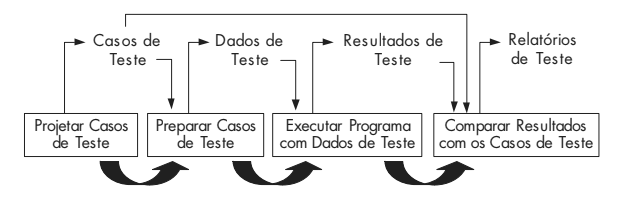
\includegraphics[width=.8\textwidth]{images/PTESTE.png}
\caption{Procedimento de Teste \cite{HIRAMA2011}}
\label{figure:PTESTE}
\end{figure}

Um dos resultados do procedimento de teste é gerar os casos de teste para que posteriormente possam ser executados.  Um bom caso de teste é aquele que tem uma grande probabilidade de revelar um defeito ainda não descoberto \cite{HIRAMA2011}.

O documento básico para a atividade de teste é o Plano de Testes, no qual se define: objetivos para cada tipo (ou fase de teste); estratégias de teste; cronograma e responsabilidades; procedimentos e padrões a serem usados na execução e na elaboração do relatório de testes; critérios para a conclusão do teste, bem como o sucesso de cada teste \cite{HIRAMA2011}.

A execução dos testes pode ser feita de forma manual, quando a partir de um roteiro a ser seguido é feita por um profissional de forma manual, ou pode ser feita de forma automatizada, com a utilização de ferramentas que execução dos testes e reportam os resultados. Para \citeonline{Ammann:2008:IST:1355340}, o teste de software é caro e exige mão de obra intensiva, e requer até 50\% dos custos de desenvolvimento de software e ainda mais para aplicativos críticos de segurança. Faz-se necessário automatizar o máximo possível dos testes de software, reduzindo significativamente o custo, minimizando o erro humano e facilitando o teste de regressão, vide Seção \ref{sec:testesregressao}.


\subsection{Técnicas de Teste de Software}


Segundo \citeonline{DELAMARO2007}, as duas técnicas mais amplamente aceitas na academia e na indústria são as técnicas de testes \textit{funcionais} e as \textit{estruturais}, comumente conhecidas como teste Caixa Preta e teste Caixa Branca, respectivamente. Elas são discutidas a seguir:



\begin{itemize}
    \item \textbf{Técnica Funcional}: Técnica utilizada para projetar casos de teste na qual o programa ou sistema é considerado uma caixa preta. Para testá-lo, fornece-se entradas e avalia-se as saídas geradas para verificar se estão em conformidade com os objetivos especificados. No teste funcional os detalhes de implementação não são considerados e o software é avaliado segundo a visão do usuário \cite{DELAMARO2007}.
    
    %\textcolor{red}{INCLUIR Particionamento em Classes de Equivalência.}%
    
    %\textcolor{red}{INCLUIR Análise do Valor Limite.}%
    
    
    \item \textbf{Técnica Estrutural}: A técnica estrutural estabelece os requisitos de teste com base em uma dada implementação, requerendo a execução de partes ou de componentes elementares do programa. Testa-se os caminhos lógicos do software, fornecendo-se casos de teste que põem à prova tanto conjuntos específicos. Os testes gerados por essa técnica são chamados também de teste de caixa branca \cite{DELAMARO2007}.
    
    %\textcolor{red}{INCLUIR Critérios Baseados em Fluxo de Controle.}%
    %\textcolor{red}{INCLUIR Critérios Baseados em Fluxo de Dados.}%
    %\textcolor{red}{INCLUIR Critérios Baseados na Complexidade.}%
    
\end{itemize}

Segundo \citeonline{HIRAMA2011}, os testes de Caixa Branca e os testes de Caixa Preta precisam atender algumas características, que são elas:\\

\textbf{Características dos testes Caixa Branca:}

\begin{itemize}
    \item O projeto de casos de teste usa a estrutura de controle procedimental do software (fluxo de controle do software) para derivar casos de teste;
    \item Deve garantir que todos os caminhos independentes dentro de um módulo tenham sido exercitados pelo menos uma vez;
    \item Deve exercitar todas as decisões lógicas para valores falsos ou verdadeiros;
    \item Deve executar todos os laços em suas fronteiras e dentro de limites operacionais;
    \item Deve exercitar as estruturas de dados internas para garantir a sua validade.
\end{itemize}



\textbf{Características dos testes Caixa Preta:}

\begin{itemize}
    \item Concentram-se nos requisitos funcionais do software;
    \item São uma abordagem complementar aos testes estruturais.
\end{itemize}


%\textcolor{red}{INCLUIR Técnicas de Teste Ágil (TDD e BDD)}%


\subsection{Tipos de Teste}


A atividade de testes é dividida em fases com objetivos distintos \cite{DELAMARO2007}. Segundo \citeonline{HIRAMA2011}, os tipos de teste mais comuns realizados para cobrir os testes estruturais e funcionais são: teste de unidade (estrutural); teste de integração (funcional); teste de validação (funcional); e teste de sistema (funcional).

\begin{itemize}

\item {\textbf{Teste de unidade}}: tem como foco as menores unidades de um programa, podendo ser funções, procedimentos, métodos ou classes. O objetivo é testar os componentes isoladamente verificando o funcionamento conjunto dos algoritmos e as estruturas de dados. Espera-se então que sejam identificados erros relacionados a algoritmos incorretos ou mal implementados, estruturas de dados incorretas, ou simples erros de programação.  A referência usada para os teste é a Especificação de Módulos, um documento detalhado de cada módulo de software. O teste de unidade pode ser aplicado à medida que ocorre a implementação das unidades e pelo próprio desenvolvedor. 

\item {\textbf{Teste de integração}}: deve ser realizado após serem testadas as unidades individuais, e a ênfase é dada na construção da estrutura do sistema. O objetivo é testar um conjunto de módulos verificando o seu funcionamento com foco nas suas interfaces entre os módulos. Quando as diversas partes do software são colocadas para trabalhar juntas, verifica-se se a interação entre elas funciona de maneira adequada e não ocasiona erros. Faz-se necessário um grande conhecimento das estruturas internas e das interações existentes entre as partes do sistema. A referência usada para os testes é a Especificação de Projeto, um documento detalhado da organização e interdependência entre os módulos de software. O teste de integração tende a ser executado pela própria equipe de desenvolvimento. 

\item {\textbf{Teste de validação}}: tem como objetivo testar o software como um todo verificando se todas as exigências funcionais, comportamentais e de desempenho foram atendidas. A referência usada para os testes é a Especificação de Requisitos de Software, um documento que contém os requisitos funcionais e não funcionais do software. O teste é realizado pela equipe de desenvolvimento de software.

\item {\textbf{Teste de sistema}}: tem como objetivo medir o sistema em diferentes cenários verificando se todos os elementos do sistema (hardware, software, banco de dados e pessoas) foram adequadamente integrados e realizam as funções requeridas. A referência usada para os testes é a Especificação de Sistema, um documento que contém a descrição funcional do sistema, dos subsistemas e do seu desempenho no ambiente operacional. O teste é realizado por uma equipe independente ou um usuário do sistema.

\end{itemize}

Segundo \citeonline{HIRAMA2011}, existem ainda outros testes que podem ser aplicados a sistemas de software. São eles: teste de recuperação, teste de proteção, teste de estresse, teste de desempenho, dentre outros, que visam validar requisitos não-funcionais do software, i.e., aqueles ligados aos atributos de qualidade esperados. Alguns desses são descritos a seguir:

\begin{itemize}
    
    \item \textbf{Teste de recuperação}: teste que força o sistema a apresentar falhas de diversas maneiras e verifica se a recuperação (reiniciação do sistema e recuperação de dados) é adequadamente executada.
    
    \item \textbf{Teste de proteção}: teste que tenta verificar se todos os mecanismos de proteção embutidos em um sistema funcionam contra acessos indevidos.
    
    \item \textbf{Teste de estresse}: teste para confrontar o software com situações anormais (alta exigência de recursos, alto número de interrupções, alta taxa de entrada de dados, alta busca de dados em disco).
    
    \item \textbf{Teste de desempenho}: teste de software no contexto de um sistema integrado (tempos envolvidos, ciclos de processador, interrupções).

\end{itemize}

Outros tipos de teste de software relevantes são os testes \textbf{alfa} e \textbf{beta}. Em virtude das dificuldades encontradas pelos desenvolvedores para preverem como o cliente usará o programa, ou, como ele irá interpretar os manuais de usuários, alguns testes são realizados para compreender como será a aceitação do cliente em relação ao software desenvolvido. 


\section{Teste de Regressão}\label{sec:testesregressao}

\subsection{Definição}

 A \citeonline{159342} define teste de regressão como repetição seletiva de um sistema ou componente para verificar se as modificações não causaram efeitos não-intencionais e se o sistema ou componentes ainda estão em conformidade com o requisito especificado. Segundo \citeonline{Ammann:2008:IST:1355340}, o teste de regressão é o processo de testar novamente o software que foi modificado. 
 
 À medida que os desenvolvedores mantêm um sistema de software, eles periodicamente fazem teste de regressão, na esperança de encontrar erros causados por suas alterações e fornecer confiança de que suas modificações estão corretas. Para suportar esse processo, os desenvolvedores geralmente criam um conjunto inicial de testes, que são reutilizáveis. A estratégia de teste de regressão mais simples é a reexecução de todos os casos de teste. Essa abordagem, porém, torna-se provavelmente inviável por exigir uma quantidade muito grande de tempo para a sua execução completa \cite{Graves:2001:ESR:367008.367020}. Para \citeonline{Ammann:2008:IST:1355340} o teste de regressão constitui a grande maioria dos esforços de teste no desenvolvimento de software comercial, e é uma parte essencial de qualquer processo de desenvolvimento de software viável.
 
 Segundo \citeonline{LEUNG1989}, os testes de regressão podem ser corretivos ou progressivos. A Tabela \ref{table:TRCP} apresenta algumas diferenças fundamentais entre ambos.

 
\begin{table}[th]
    \footnotesize
    \centering
    \caption{Teste de Regressão Corretivo \& Progressivo \cite{LEUNG1989}}
    \label{table:TRCP}
    \def \arraystretch{1.3}
    \begin{tabular}{m{6.5cm}m{6.5cm}}
        \toprule
        \textbf{Teste de Regressão Corretivo} & \textbf{Teste de Regressão Progressivo} \\
        \midrule
        \textit{A especificação não é alterada} & A especificação é alterada\\
        \textit{Envolve pequenas modificações no código (por exemplo, adicionar e excluir instruções)} & Envolve modificação importante (por exemplo, adicionar e excluir módulos)\\ 
        \textit{Geralmente feito durante o desenvolvimento e a manutenção corretiva} & Geralmente feito durante a manutenção adaptativa e aperfeiçoada\\
        \textit{Muitos casos de teste podem ser reutilizados} & Menos casos de teste podem ser reutilizados\\
        \textit{Chamado em intervalos irregulares} & Chamado em intervalos regulares\\
        \bottomrule
    \end{tabular}
\end{table}

Para \citeonline{Ammann:2008:IST:1355340}, os testes de regressão devem ser automatizados. De fato, pode-se dizer que o teste de regressão não automatizado é equivalente a nenhum teste de regressão.


\subsection{Distinção entre as classes de técnicas}
 
Para \citeonline{Ammann:2008:IST:1355340} uma técnica é \textbf{precisa} na medida em que omite testes de regressão que não são reveladores de modificação. Uma técnica é \textbf{eficiente} na medida em que determinar o subconjunto apropriado do conjunto de testes de regressão. E, uma técnica é \textbf{geral} no grau que se aplica a uma ampla variedade de situações práticas.

Segundo \citeonline{Yoo:2012:RTM:2284811.2284813} as técnicas de teste de regressão são classificadas como: Técnicas de Seleção; Técnicas de Minimização; e Técnicas de Priorização, seguida das seguintes definições:
 
 
\begin{itemize}
 
 \item \textbf{Definição 1 (Problema de Minimização do Conjunto de Testes)}:
 
 As técnicas de minimização do conjunto de testes visam identificar casos de teste redundantes e removê-los do conjunto de testes para reduzir o tamanho do conjunto de testes.
  
\textbf{Dado}: Um conjunto de testes $T$, um conjunto de requisitos de teste ${r1, ..., rn}$, que deve ser satisfeito para fornecer o teste ``adequado'' desejado do programa e subconjuntos de $T, T1, ..., T_n$, um associado a cada um dos $r_is$ de tal forma que qualquer um dos casos de teste $t_j$ pertencentes ao $T_$ pode ser usado para atingir o requisito $r_i$.

\textbf{Problema}: Encontre um conjunto representativo, $T'$, de casos de teste de $T$ que satisfaça todos os $r_is$.



\item \textbf{Definição 2 (Problema de Seleção de Casos de Teste)}:

A seleção do caso de teste, no inglês \ac{RTS}, é essencialmente semelhante ao problema de minimização do conjunto de testes: ambos os problemas tratam da escolha de um subconjunto de casos de teste do conjunto de testes. A principal diferença entre essas duas abordagens na literatura é se o foco está nas mudanças no \ac{SUT}, em português, sistema sob teste. A minimização do conjunto de testes geralmente é baseada em métricas como a cobertura medida de uma única versão do programa em teste. Em contraste, no \ac{RTS}, os casos de teste são selecionados porque sua execução é relevante para as mudanças entre a versão anterior e a atual do \ac{SUT}.

\textbf{Dado}: O programa $P$, a versão modificada de $P$, $P'$ e um conjunto de testes $T$.
\textbf{Problema}: Encontre um subconjunto de  $T$ , $T'$, com o qual testar $P'$.



\item \textbf{Definição 3 (Problema de Priorização de Casos de Teste)}:

A priorização de caso de teste procura encontrar o pedido ideal de casos de teste para teste, para que o testador obtenha o máximo benefício, mesmo se o teste for prematuramente interrompido em algum ponto arbitrário. 

\textbf{Dado}: Um conjunto de testes $T$, o conjunto de permutações de $T$, $PT$ e uma função de $PT$ para números reais, $f: PT \longrightarrow R$.

\textbf{Problema}: Para encontrar $T' \in PT \longrightarrow (\forall T")(T" \in PT)(T" \ne T')[f(T') \geq  f(T")]$.


\end{itemize}


\subsection{Classificação dos Casos de Testes}


Segundo \cite{Yoo:2012:RTM:2284811.2284813} categorizam os casos de teste em cinco classes. As três primeiras classes consistem em casos de teste que já existem em $T$.

\begin{itemize}
  \item \textbf{Reutilizável}: Os casos de teste reutilizáveis executam apenas as partes do programa que permanecem inalteradas entre duas versões, ou seja, as partes do programa que são comuns a $P$ e $P'$. Não é necessário executar esses casos de teste para testar $P'$; no entanto, eles são chamados de reutilizáveis porque ainda podem ser retidos e reutilizados para o teste de regressão das futuras versões do $P$.
  \item \textbf{Retestável}: Casos de teste retestáveis executam as partes de P que foram alteradas em $P'$. Assim, os casos de teste retestáveis devem ser reexecutados para testar $P'$.
  \item \textbf{Obsoleto}: Os casos de teste podem se tornar obsoletos porque (1) sua relação de entrada / saída não é mais correta devido a mudanças nas especificações, (2) eles não testam mais o que foram projetados para testar devido a modificações no programa ou (3) casos de teste ``estruturais'' que não mais contribuem para a cobertura estrutural do programa.

As duas classes restantes consistem em casos de teste que ainda precisam ser gerados para o teste de regressão de $P'$.

\item \textbf{Novo-estrutural}: Novos casos de teste estrutural testam as construções modificadas do programa, fornecendo cobertura estrutural das partes modificadas em $P'$.


\item \textbf{Nova especificação}: Casos de teste de nova especificação testam as especificações do programa modificado, testando o novo código gerado a partir das partes modificadas das especificações de $P'$.
\end{itemize}

\section{Técnicas de seleção de teste de regressão}\label{sec:rts}


Em virtude da necessidade de técnicas \textbf{eficientes}, que determinam o subconjunto apropriado de casos de testes a serem reexecutados, e de técnicas \textbf{precisas} que omitem casos de testes que não são reveladores de modificação \cite{Ammann:2008:IST:1355340}, ao longo de décadas diversos estudos são realizados para prover essas técnicas \cite{WHITE1991}, \cite{Graves:2001:ESR:367008.367020}, \cite{630875}, \cite{536955}, \cite{ENGSTROM201014},\cite{ENGSTROM201014}, \cite{KAZMI2017}, \cite{ROMANO201862}.

As técnicas podem ser categorizadas, para que sejam avaliadas e comparadas, em quatro categorias: inclusividade, precisão, eficiência e generalidade. A \textbf{inclusividade} mede o quanto uma técnica escolhe testes que farão com que o programa modificado produza uma saída diferente do programa original expondo falhas causadas por modificações. A \textbf{precisão} mede a capacidade de uma técnica evitar a escolha de testes que não farão com que o programa modificado produza resultados diferentes do programa original. A \textbf{eficiência} mede o custo computacional e, portanto, a praticidade de uma técnica. A \textbf{generalidade} mede a capacidade de uma técnica lidar com construções de linguagem realistas e diversificadas, modificações de código arbitrariamente complexas e aplicativos de teste realistas \cite{536955}.

As técnicas de seleção reduzem o custo do teste de um programa modificado, pois, reutilizam testes existentes e identificam partes do programa modificado ou sua especificação que deve ser testada. Estas técnicas diferem da técnica de reexecução de todos os casos de teste da versão original. Segundo \cite{WHITE1991}, uma técnica de seleção é mais econômica que a técnica de reexecução de todos os casos de teste, se o custo de selecionar um subconjunto reduzido de testes a executar for menor que o custo de executar os testes que a técnica de seleção omitir.

Os procedimentos fundamentais executados por uma técnica de seleção de teste de regressão são: \cite{536955}

\begin{enumerate}
    \item Selecionar $T'$ $\subseteq$ $T$, um conjunto de casos de testes para executar em $P'$.
    \item Testar $P'$ com $T'$, para estabelecer a correção de $P'$ em relação a $T'$.
    \item Se necessário, criar $T''$, um novo conjunto de casos de teste funcional ou estrutural para testar $P'$.
    \item Testar $P'$ com $T''$, para estabelecer a correção de $P'$ em relação a $T''$.
    \item Crie $T'''$, um novo conjunto de casos de testes e histórico de testes para $P'$, de $T$, $T'$, e $T''$.
\end{enumerate}

Executando essas etapas, uma técnica de seleção de teste de regressão aborda quatro problemas. A etapa 1 refere-se ao problema de selecionar um subconjunto de testes $T'$ de $T$ com o qual possa testar $P'$. A etapa 3 refere-se ao problema de cobertura, ou seja, identificar a necessidade de criação de testes adicionais. As etapas 2 e 4 tratam o problema de executar testes com eficiência, verificando se os resultados estão corretos. A etapa 5 refere-se ao problema de manutenção do conjunto de testes, atualizando e armazenando as informações de teste.

As técnicas de seleção de teste de regressão tem como foco o problema 1, ou seja, selecionar um subconjunto de teste de $T$, $T'$ com o qual testar $P'$, garantindo assim que as mudanças realizadas não modificaram o funcionamento do software. Essas técnicas localizam testes em $T$ que expõem falhas em $P'$.

Algumas premissas fundamentais em relação a técnicas de seleção de teste de regressão: \cite{536955}
\begin{itemize}
    \item Um teste $t$ detecta uma falha em $P'$ se ele faz com que $P'$ falhe. Neste caso pode-se dizer que $t$ é um revelador de falhas de $P'$.
    \item Um programa $P$ falha em $t$ se, quando $P$ for testado com $t$, $P$ produzir uma saída incorreta de acordo com $S$.
    \item Uma técnica de seleção de teste de regressão pode selecionar um subconjunto do conjunto de testes em $T$ que revelam falhas para $P'$. Nessas condições pode-se dizer que essa técnica não omite testes em $T$ que possam revelar falhas em $P'$.
    \item Um teste $t$ é revelador de modificações para $P$ e $P'$ se, e somente se, faz com que as saídas de $P$ e $P'$ sejam diferentes.
    \item O teste $t$ é considerado obsoleto para o programa $P'$ se e somente se $t$ especificar uma entrada para $P'$ que, de acordo com $S'$, é inválida para $P'$ ou $t$ especificar uma relação de entrada-saída inválida para $P'$.
\end{itemize}

A literatura apresenta diversos estudos sobre técnicas de seleção de teste de regressão, tais como, revisões sistemáticas, \textit{survey}, estudos empíricos: \cite{WHITE1991}, \cite{536955}, \cite{630875}, \cite{Rosenblum97acomparative}, \cite{Rothermel2000},  \cite{Graves:2001:ESR:367008.367020},    \cite{ENGSTROM201014}, \cite{KAZMI2017}, \cite{ROMANO201862}.

\section{Testes de apps para Android}\label{testesAndroid}

Segundo \citeonline{glauber2019dominando} o Android não é apenas um sistema operacional, mas um conjunto completo de software para dispositivo móveis que inclui: um sistema operacional, um \textit{middleware} e aplicações-chave. O Android é open-source e seu código fonte está disponível para download \footnote{\url{https://source.android.com/}}. Assim como o código-fonte, a documentação para desenvolvimento e teste também está disponível para consulta\footnote{\url{https://developer.android.com/}} . 

Desenvolver e testar apps para Android apresentam alguns desafios específicos, tais como: concorrência, segurança, performance, eficiência energética, compatibilidade, detecção de defeitos \cite{8453877}. Assim, testar um app para Android é uma tarefa que tende a exigir um esforço da equipe. 

Com o objetivo de reduzir o esforço de teste no processo de desenvolvimento de apps para Android, tanto a literatura, quanto o mercado, propõe ferramentas para automatizar o processo de testes em \ac{APPS} Android. As ferramentas podem ser gratuitas ou proprietárias, e estão focadas em diferentes tipos de testes no processo de desenvolvimento dos apps conforme \ref{table:androidtools}.

\section{Síntese do Capítulo}\label{sec:sintesecapitulo}

O presente capítulo apresentou os conceitos fundamentais para compreensão do estudo proposto. Na Seção \ref{sec:evolucaodesoftware} abordamos sobre o processo de evolução de software. Na Seção \ref{sec:qualidadedesoftware} definimos o conceito de qualidade e sua importância no processo de desenvolvimento de software. A Seção \ref{sec:testesdesoftware} apresenta diversos conceitos sobre teste de software. Na Seção \ref{sec:testesregressao} tratamos sobre uma técnica distinta de testes, denominada teste de regressão. Na Seção \ref{sec:rts} tratamos sobre as técnicas de seleção de teste de regressão. E na Seção \ref{testesAndroid} abordarmos sobre a atividade de testes em apps para Android.
\xchapter{\textit{Survey}}{}

\acresetall 

Com o objetivo de compreender como testadores e desenvolvedores, realizam o teste de regressão, e como forma de responder a QP3 da presente investigação, aplicamos um \textit{Survey}, que foi respondido por 100 profissionais e pesquisadores que atuam em projetos de \ac{APPS} para Android. Neste capítulo, encontram-se detalhes sobre o planejamento, execução e resultados obtidos.
Os resultados obtidos com a aplicação deste \textit{Survey} foram reportados em um artigo submetido e aceito pelo SBES 2020 - Trilha de Ideias Inovadoras e Resultados Emergentes.


\section{Apresentação e Questões de Pesquisa}\label{rqsurvey}

Segundo \cite{PSK2001} um \textit{survey} é um sistema abrangente que tem como objetivo coletar informações para descrever, comparar ou explicar conhecimentos, atitudes e comportamentos. %A literatura apresenta alguns trabalhos que tem trazem a aplicação de teste de regressão na indústria \cite{Ali2019}, \cite{8094467}, \cite{7102609}, \cite{630875}.%

Definimos as seguintes Questões de Pesquisa (RQ):

\begin{enumerate}[label=\bf QP\arabic*,leftmargin=1.8cm]
    
    \item \textbf{Quão automatizado é o teste de regressão de aplicativos Android na prática?} Esta questão de pesquisa tem como objetivo identificar se os testadores utilizam-se de ferramentas para testar aplicativos Android. Também deseja-se descobrir as ferramentas usadas.
    
    \item \textbf{Como é realizado o processo de teste durante e após a manutenção dos \ac{APPS}?} Esta questão de pesquisa tem como objetivo identificar se os testadores realizam teste de regressão, e com que frequência. Também procura-se entender se e quais estratégias de seleção de teste podem ser empregadas para reduzir a quantidade de testes reexecutados.
    
    \item \textbf{Quais são os motivos para não realizar testes de regressão após a manutenção de \ac{APPS} para Android?} Esta questão de pesquisa tem como objetivo entender os motivos pelos quais os testadores não realizam testes de regressão em sua prática.
    
\end{enumerate}

\section{Metodologia de Pesquisa}\label{rmsurvey}

Este \textit{Survey} tem como objetivo compreender como testadores e desenvolvedores, realizam o teste de regressão em projetos de \ac{APPS} para Android.

Esta seção abrange os detalhes do planejamento, procedimentos de execução e relatórios dos resultados desejados e alcançados. Utilizamos a metodologia proposta por Kasunic \cite{Kasunic2005DesigningAE} e aplicamos os princípios de pesquisa definidos por Kitchenham et al. \cite{Kitchenham:2002:PSR:566493.566495}.


\subsection{Identificação do Público Alvo}

Para obter resultados válidos, selecionamos como público-alvo estudantes e profissionais de diferentes estados do Brasil que trabalham com testes de aplicativos para Android. 


\begin{comment}
Foram considerados três critérios:

\begin{enumerate}
    \item Pessoas que trabalham de forma autônoma; 
    \item Pessoas que trabalham / pesquisam em uma empresa; 
    \item Alunos pesquisando tópicos relacionados.
\end{enumerate}

\end{comment}

\subsection{Design do Questionário}


O \textit{Survey} é dividido em quatro seções. A Seção I refere-se ao termo de consentimento livre e esclarecido. A seção II refere-se à identificação do participante, a qual consiste em 13 perguntas, a maioria das quais são obrigatórias (8 perguntas de múltipla escolha, 3 subjetivas e 2 de seleção). Essas perguntas se referem a informações demográficas, área de formação, conhecimento e experiência em testes de software e testes de aplicativos Android. A Seção III trata do processo de teste de aplicativos Android. Consiste em 16 perguntas, a maioria das quais são obrigatórias (7 perguntas de múltipla escolha, 3 perguntas subjetivas e 6 perguntas na caixa de seleção). Essas perguntas tratam de como o processo de teste de software é realizado pelos participantes, bem como o uso de ferramentas para automatizar o processo de teste e se eles estão ou não satisfeitos com as ferramentas existentes. Finalmente, a Seção IV refere-se às considerações finais. 87\% das perguntas eram obrigatórias. A seguir, descrevemos os objetivos de cada seção do questionário.


\begin{itemize}
    \item \textbf{Perfil dos entrevistados:} pretendemos identificar o perfil dos entrevistados, com informações sobre sexo, idade, escolaridade, área de formação, certificações de teste, nível de conhecimento e experiência em testes de software e, especificamente, em aplicativos Android.
    
    \item \textbf{Foco da atividade de teste:} procuramos identificar se os testes realizados são funcionais ou estruturais. Além disso, queremos identificar os tipos de testes realizados nos projetos atuais, como: teste de \ac{GUI}, teste de unidade, teste de integração, teste de regressão, etc.
    
    \item \textbf{Automação do processo de teste:} pretendemos identificar se os testes são realizados de forma manual ou automatizada. Além disso, queremos identificar o suporte ferramental utilizado pelos entrevistados. No questionário, listamos ferramentas para testar aplicativos Android, encontradas na literatura e aplicadas na indústria. Portanto, poderíamos investigar se as ferramentas listadas na literatura também são conhecidas e utilizadas pelos entrevistados. A Tabela \ref{table:androidtools} do Apêndice A mostra o conjunto de ferramentas de teste para aplicativos Android sobre as quais perguntamos aos entrevistados.
    
    \item \textbf{Processo de teste de regressão:} pretendemos identificar se os nossos participantes realizam testes de regressão após realizar manutenção em aplicativos Android. Estamos interessados em descobrir se: (i) o processo é feito manualmente ou automatizado; (ii) é aplicada alguma técnica de seleção de caso de teste; (iii) são utilizadas ferramentas, encontradas na literatura ou aplicadas na indústria; (iv) se estão satisfeitos com as ferramentas existentes; e (v) se e por que consideram a execução de testes de regressão como relevante.
    
\end{itemize}

\subsection{Projeto Piloto}

Aplicamos um piloto com três participantes, dois profissionais e um pesquisador, todos trabalhando com testes de aplicativos Android. Para a versão piloto do questionário, adicionamos uma seção de avaliação em que os participantes puderam fazer contribuições sobre a estrutura do questionário e indicar sugestões de melhorias. A seção de avaliação apresentou questões relacionadas à adequação das questões em relação ao tema da pesquisa; o número de perguntas a serem respondidas; o tempo necessário para responder ao formulário; e a relevância da pesquisa, como segue:


\begin{enumerate}
    \item Em uma escala de 1 a 5, onde 1 é igual a ruim e 5 é igual a ótimo, como você avalia o número de perguntas no formulário?
    \item Em uma escala de 1 a 5, onde 1 é igual a ruim e 5 é igual a ótimo, como você avalia a adequação das perguntas do formulário ao tema ``Processo de teste de aplicativos para Android"?
    \item Cite pontos para melhorias.
    \item Cite pontos positivos do questionário.
    \item Deixe um comentário sobre o questionário.
\end{enumerate}

O \textit{feedback} sugeriu pequenas modificações na estrutura do questionário. As mudanças incluíram: adicionar opções de resposta a várias perguntas, alterar palavras para melhorar o entendimento e destacar o objetivo da pergunta para diferenciar questões que têm contextos semelhantes. Com base nas melhorias identificadas, uma segunda versão do questionário foi gerada.


\subsection{Distribuição do Questionário}

Para criar o questionário, usamos a ferramenta online Formulários Google\footnote{\url{http://docs.google.com/forms}}. O processo de ampla divulgação desta pesquisa foi realizado em 20 de janeiro de 2020 e ficou disponível por aproximadamente dois meses no primeiro semestre de 2020. O link do questionário foi enviado por e-mails (individuais e listas de e-mail) e mídias sociais, como o Linkedln. %O questionário também foi enviado por e-mail para empresas que trabalham com o desenvolvimento de aplicativos Android.%
O formulário foi enviado juntamente com um texto de convite, com informações essenciais sobre o objetivo do estudo e a importância do estudo. Os participantes também foram informados sobre as políticas de privacidade do estudo de maneira clara e detalhada.


\section{Resultados}\label{resultssurvey}

O \textit{Survey} recebeu 106 respostas, sendo que 6 destas foram descartadas, pois os entrevistados não tinham experiência anterior com teste de software nem trabalhavam com projetos de aplicativos Android, ou por terem respondido o formulário de forma duplicada, totalizando 100 respostas para análise. 

\subsection{Perfil dos entrevistados}

Quanto ao sexo e a idade dos entrevistados, 81\% eram homens e 19\% mulheres; A maioria deles 66\% tinha entre 20 e 30 anos (29\% de 20 a 25 e 37\% de 26 a 30 anos); 22\% tinham entre 31 e 35 anos; e 12\% tinham mais de 35 anos. 

Quanto ao nível de escolaridade, 9\% tinham apenas o ensino médio completo; 5\% tinham curso técnico; 7\% eram estudantes de graduação; 55\% eram graduados; 1\% era estudante de pós-graduação e 23\% possuíam diplomas mais altos, como MBA, mestrado. ou um Ph.D. Além disso, a maioria dos entrevistados possuía diploma em Ciência da Computação ou cursos relacionados (89\%); 9\% eram formados em engenharia elétrica ou engenharia de produção; e 2\% possuíam diplomas em outras áreas. Ao considerar certificações ou cursos na área de teste de software, 56 dos 100 participantes possuíam pelo menos um certificado em cursos de teste de software, como o CTFL \textit{(Certified Tester Foundation Level)} e o \textit{Certified in Tester Foundation Level - Agile Tester (CTFL-AL)}.

Ao considerar a procedência dos entrevistados, a maioria eram estudantes e/ou profissionais (81\%) que atuam em uma empresa; 21\% eram estudantes e 18\% eram profissionais autônomos. Em termos de experiência profissional em teste de software, a maioria deles possuía até 5 anos de experiência e apenas 7\% possuía mais de 10 anos de experiência. No entanto, quando perguntados especificamente sobre sua experiência no teste de aplicativos Android, quase metade dos entrevistados (48\%) tinha apenas 1 ano de experiência. Além disso, quando questionados sobre seu nível de conhecimento em testar aplicativos Android em comparação com outros profissionais, quase metade deles considerou seu nível bom ou excelente, e 29\% deles consideraram baixo ou muito baixo, como mostra a Tabela 2.
 
Em relação à posição principal do projeto atual na empresa, os entrevistados consideraram uma das seguintes descrições: analista de qualidade, desenvolvedor, analista de teste, desenvolvimento móvel com Android, desenvolvedor, desenvolva para Android, analista de sistemas, gerente de projeto, gerente técnico e engenheiro de teste.
 
Com relação às principais tarefas, 72\% dos entrevistados trabalham com criação e design de caso de teste e 85\% deles trabalham apenas com execução de caso de teste.

\begin{table*}[htbp]
\centering
  \def \arraystretch{1.1}
  \footnotesize
  \caption{Resumo do nível de experiência dos respondentes}
    \begin{tabular}{ccccc}
    \toprule
    \multicolumn{5}{l}{\textbf{Experiência profissional em testes de softwares (em anos)}} \\
    \midrule
    \textbf{$<$1} & \textbf{1-3} & \textbf{3-5} & \textbf{5-10} & \textbf{$>$10} \\
    \midrule
    23\%  & 30\%  & 21\%  & 19\%  & 7\% \\
    \midrule
    \multicolumn{5}{l}{\textbf{Experiência em testes de \ac{APPS} Android (em anos)}} \\
    \midrule
    \multicolumn{1}{c}{\textbf{$<$1}} & \textbf{1-3} & \textbf{3-5} & \textbf{5-10} & \textbf{$>$10} \\
    \midrule
    48\%  & 25\%  & 17\%  & 10\%  & {\textbf{-}} \\
    \midrule
    \multicolumn{5}{m{10cm}}{\textbf{Nível de conhecimento em testes de \ac{APPS} Android quando comparado a outros profissionais}} \\
    \midrule
    \textbf{Muito baixo} & \textbf{Baixo} & \textbf{Regular} & \textbf{Bom} & \textbf{Ótimo} \\
    \midrule
    7\%   & 22\%  & 23\%  & 34\%  & 14\% \\
    \bottomrule
    \end{tabular}%
  \label{tab:professionalinformation}%
\end{table*}

\subsection{Questões de Pesquisa}

Em seguida, relatamos os resultados da pesquisa, com base no conjunto das questões de pesquisa apresentadas anteriormente na na Seção \ref{rqsurvey}.

\begin{enumerate}[label=\bf QP\arabic*]
    
\item \textbf{Quão automatizado é o teste de regressão de aplicativos Android na prática?}
    
Os entrevistados foram perguntados se eles costumavam executar testes de forma manual, automatizada ou se usavam as duas abordagens. 52\% dos entrevistados indicaram que adotam testes automatizados e manuais. Além disso, 30\% dos entrevistados responderam que realizam apenas testes manuais; e 18\% seguem um processo de teste suportado por ferramentas.
 
Em outra questão sobre o uso de ferramentas, 35\% dos entrevistados informaram que não usam ferramentas para testar seus aplicativos. No entanto, essa resposta contrasta com a anterior, quando 30\% afirmaram que só realizam testes manualmente. Em relação às ferramentas usadas com frequência, as mais relatadas foram Appium, Espresso, UI Automator, Roboeletric e Monkey. Todas essas ferramentas são gratuitas.
 
Também perguntamos aos entrevistados se eles usam ferramentas para realizar testes de regressão. 67\% deles não usam nenhuma ferramenta específica. 11\% dos entrevistados afirmaram não testar aplicativos após a manutenção e 29\% usam nenhuma ferramenta após a manutenção ou atualização, da seguinte forma: 13\% usam as mesmas ferramentas adotadas para testes regulares para realizar testes de regressão; 12\% usam ferramentas específicas de teste de regressão, conforme indicado na literatura; e 4\% usam outras ferramentas, como TestNG\footnote{\url{https://testng.org/doc/}} e ferramentas internas, ou seja, aquelas desenvolvidas por sua própria empresa.

Perguntamos aos participantes como eles poderiam avaliar a relevância do suporte de ferramentas existente para testes de regressão, no sentido de que eles poderiam indicar se as ferramentas poderiam atender às suas necessidades específicas ou não.

Para 10\% dos entrevistados, as ferramentas nunca atendem às suas necessidades. Para 8\%, elas raramente atendem às suas necessidades. Para 13\%, as ferramentas às vezes atendem às suas necessidades. Para 24\%, eles geralmente atendem às suas necessidades. 18\% dos participantes responderam que as ferramentas sempre atendem às suas necessidades e 27\% dos participantes não testam o aplicativo após a manutenção.
    
\item \textbf{Como é realizado o processo de teste durante e após a manutenção dos \ac{APPS}?:}

Para 51\% dos entrevistados, é ``sempre'' necessário testar novamente os aplicativos Android após a manutenção ou atualização para garantir que a manutenção realizada não altere o comportamento funcional do aplicativo. Para os outros entrevistados, 20\% responderam que ``às vezes'' testam, 19\% ``frequentemente'', 6\% ``raramente'' e apenas 4\% ``nunca''.

Os entrevistados também foram questionados sobre os procedimentos de teste que geralmente executam após a manutenção. A questão de pesquisa tem como objetivo entender se os participantes usaram estratégias para reduzir a quantidade de execuções de casos de teste preexistentes. A maioria dos entrevistados (77\%) seleciona e reutiliza os casos de teste que se referem às alterações entre a versão original e a versão atualizada do aplicativo Android. Essa estratégia pode reduzir o tempo necessário para testar o aplicativo. No entanto, 59\% responderam que reexecutam todos os casos de teste da versão original para testar a versão atualizada do aplicativo Android. 58\% dos entrevistados analisam se é necessário criar novos casos de teste para a versão atualizada do aplicativo. 10\% deles excluem um conjunto de casos de teste que não detectam falhas na versão atualizada do aplicativo Android. Vale ressaltar que nesta pergunta em particular, os entrevistados podiam selecionar mais de uma opção.

    
\item \textbf{Quais são os motivos para não realizar testes de regressão após a manutenção de \ac{APPS} para Android?}

Embora 11\% dos entrevistados não realizem testes após a manutenção ou atualização de software, 99\% consideraram essa tarefa relevante.
 
Portanto, os entrevistados foram questionados sobre os principais motivos pelos quais as empresas não testam aplicativos após a manutenção. Para 71\%, o tempo de entrega reduzido para o lançamento do novo aplicativo é o motivo mais relatado. 28\% dos entrevistados responderam que o problema se deve ao alto esforço da equipe de teste; para 23\%, a detecção de erros na nova versão tem pouca importância; 22\% dos entrevistados responderam que o motivo é a falta de um processo suportado por ferramentas.

Além disso, os entrevistados também compartilharam suas opiniões, com declarações como ``temos uma cultura no processo de desenvolvimento, que acreditamos que a fixação de uma área não afetará outra'' e ``os clientes geralmente pressionam a equipe para lançar o produto no mercado para não perder o tempo de colocação no mercado''.



\end{enumerate}

\section{Discussões}\label{discussions}

Nesta seção, discutimos os resultados em três aspectos: foco da atividade de teste, automação do processo de teste, e entender o processo de teste de regressão.

\begin{itemize}
\item \textbf{Foco da atividade de teste:} Os resultados indicaram que os entrevistados realizam mais testes funcionais, nos quais não precisam acessar o código-fonte do aplicativo. Além disso, o estudo mostrou que os funcionários executam principalmente testes de validação, testes de integração, testes de sistema, testes de regressão, testes de interface gráfica do usuário (GUI) e testes de unidade. Esses testes podem ser essenciais para garantir a qualidade do aplicativo. Por exemplo, os testes da GUI podem ser um item indispensável para a qualidade de um aplicativo; O teste de validação verifica se o sistema atende aos requisitos solicitados. Com relação à preferência por testes funcionais em vez de não funcionais, pode ser necessário atrair especialistas em tecnologias de software e código fonte específicos para realizar testes não funcionais. Além disso, ferramentas podem ser adotadas para facilitar a execução e criação do teste.

Pesquisas futuras poderão ser realizadas para entender: (i) a relação entre os tipos de testes (validação, unidade, GUI, sistema) e o quão são automatizados; (ii) as abordagens e estratégias usadas para realizar testes funcionais ou não funcionais; e (iii) quais razões levam os profissionais a escolher uma técnica de teste específica em detrimento de outra.
    
\item \textbf{Automação do processo de teste:} A automação dos testes não é executada na maioria das empresas de software pesquisadas, apenas 18\% dos participantes realizam testes automatizados. No entanto, eles poderiam reduzir significativamente o custo do processo de teste, minimizar o erro humano e facilitar o teste de regressão \cite{Ammann:2008:IST:1355340}. Portanto, o desenvolvimento de ferramentas apropriadas pode trazer grandes benefícios para a área.

Além disso, a maioria dos entrevistados usa ferramentas gratuitas, que supostamente não atendem totalmente às suas necessidades profissionais. Além disso, as ferramentas acadêmicas podem ter poucos requisitos e não são disponíveis para uso comercial.

Uma pesquisa ou comparação da eficácia das ferramentas de teste pode ser realizada para orientar e auxiliar os testadores durante as atividades de teste. Neste estudo, também perguntamos aos participantes sobre quais recursos poderiam ser aprimorados ou implementados nas ferramentas que eles estão usando atualmente.

As respostas mais relevantes foram:

\begin{itemize}
    \item ``Os testes de UI no Android ainda são difíceis e demorados para construir.''
    \item ``A criação e execução das suítes de teste precisam ser automatizadas para permitir uma verificação mais rápida da qualidade da aplicação frente a alterações.''
    \item ``Acho que poderia ser emitido relatórios de tempo de execução de testes em relação a uma versão anterior e informar se teve algum caso de teste que não foi coberto na nova versão e que estava sendo coberto na versão anterior.''
    \item ``Serem mais \textit{User Friendly}.''
    \item ``Dificilmente uma ferramente vai conseguir fornecer tudo que o projeto precisa em relação a testes, então não acho que seja uma feature/funcionalidade que venha a resolver todos os problemas. O que a equipe realmente precisa ter é uma pessoa que entenda de testes e que quando falta alguma coisa em alguma ferramenta pronta, consegue mobilizar a equipe para criar uma lib do zero para resolver aquele problema. Isto é bem melhor do que ficar importando várias ferramentas de teste para o projeto, porque naturalmente cada uma é melhor em um aspecto. Então chega um certo ponto, que ao invés de ficar experimentando ferramentas novas para ver se resolve um problema, é melhor a equipe desenvolver esta nova ferramenta.''
    
\end{itemize}

Tais respostas apresentam dificuldades encontradas pelos participantes no uso de ferramentas de teste automatizadas para aplicativos Android, que representam alguns dos motivos pelos quais eles não costumam usar as ferramentas existentes. Estudos futuros podem ser feitos para mapear a relação entre automação e tipo de teste, para que se possa entender: (i) quais tipos de testes mais exigem ferramentas; e (ii) quais recursos são esperados por esses profissionais para cada tipo específico de teste.
    
\item \textbf{Processo de teste de regressão:} 

Embora 99\% dos participantes considerem relevante para realizar testes de regressão, a quantidade de profissionais que realmente os realiza é muito menor. A seleção dos testes mais adequados pode reduzir o custo do software e o esforço da equipe. Além disso, a pesquisa não incluiu a palavra regressão em nenhuma pergunta ou resposta. Assim, alguns dos entrevistados podem não ter entendido que testar o aplicativo após executar sua atualização (manutenção) se refere a testes de regressão \cite{LEUNG1989}. Observamos divergências nas respostas dos entrevistados. Por exemplo, quando perguntados se eles realizam algum tipo de teste após a manutenção do aplicativo (atualização) para garantir que as alterações não afetem o comportamento funcional do aplicativo, 4\% responderam que nunca realizam esses testes. No entanto, em uma pergunta relacionada, 12\% responderam que não testam o aplicativo após a manutenção.
 
Embora a literatura apresente muitos estudos sobre técnicas de seleção de casos de teste como uma maneira de reduzir a quantidade de casos de teste no processo de teste de regressão \cite{KAZMI2017,ENGSTROM201014, 536955, WHITE1991,LEUNG1989}, muitos profissionais ainda reexecutam todos os casos de teste como na última versão. Como a maioria dos entrevistados não usa o suporte de ferramentas, o custo e o esforço para aplicar uma estratégia de seleção manualmente podem ser maiores do que reexecutar o conjunto completo de testes. Estes resultados reforçam a necessidade de ferramentas que forneçam uma seleção adequada de casos de teste. Estudos futuros são necessários para confirmar esses resultados preliminares.

\end{itemize}


\section{Ameaças à Validade}\label{threatstovalidity}

\textbf{Validade interna:} A pesquisa foi desenhada por um pesquisador e revisada por três pesquisadores. Posteriormente, um projeto piloto foi aplicado para validação. Além disso, as respostas dos respondentes foram dadas em português e o relato foi feito em inglês. Para mitigar essa ameaça, realizamos a tradução em pares, buscando manter a confiabilidade dos dados coletados.

\textbf{Validade externa:} Embora este estudo seja baseado em uma amostra que considerou pesquisadores e profissionais de teste de software, os resultados não podem ser generalizados para outros cenários. No entanto, este estudo é um passo inicial para fornecer mais evidências sobre a consciência e percepção dos profissionais sobre o uso de teste de regressão na manutenção de aplicativos Android. 

\textbf{Validade de construção:} No questionário,  evitamos usar o termo teste de regressão. Em vez disso, usamos implicitamente a definição do teste de regressão como uma estratégia para evitar viés e impedir que os participantes pesquisassem o conceito, antes de responder ao questionário. Apesar dos esforços, alguns participantes podem não ter relacionado a definição ao teste de regressão.


\section{Síntese do capítulo}

O presente capítulo apresentou o \textit{Survey} utilizado como instrumento de pesquisa para compreender qual a perspectiva de acadêmicos e profissionais sobre técnicas de seleção de teste de regressão implementadas por ferramentas para projetos de \ac{APPS} Android. Na Seção \ref{rqsurvey} definimos as questões de pesquisa. Na Seção \ref{rmsurvey} apresentamos a metodologia utilizada. A Seção \ref{resultssurvey} apresenta os resultados obtidos. Na Seção \ref{discussions} as devidas discussões, e na seção \ref{threatstovalidity} as ameaças à validade.





























\xchapter{Considerações Finais}{}
\acresetall
São apresentados neste capítulo os trabalhos relacionados, e os próximos passos desta investigação científica.

\section{Trabalhos Relacionados}

Nesta seção serão apresentados os trabalhos relacionados a este estudo. A literatura apresenta alguns trabalhos referentes à técnicas de teste de regressão para Android:

\begin{itemize}
    
    \item \cite{8377661}: Este trabalho apresenta um estudo sobre técnicas de seleção de teste de regressão. Os pesquisadores propõem a criação de uma técnica denominada \textbf{ReTestDroid} que serve para modelar invocações de tarefas assíncronas, ciclo de vida de atividades baseado em fragmentos e código nativo dentro do gráfico de fluxo de controle de uma aplicação Android. A técnica é implementada e testada em cinco \ac{APPS} Android.
    
    \item \cite{Do2016RedroidAR}: Este trabalho apresenta um estudo de \textit{bugs} reais em \ac{APPS} Android que demonstra a existência de erros de regressão. Como solução para este problema, os pesquisadores propõem a técnica de seleção de teste de regressão denominada \textbf{REDROID} que aproveita a combinação de análise de impacto estático e cobertura dinâmica de código, para identificar um subconjunto de casos de teste para re-execução na versão modificada do aplicativo. A técnica foi implementada e testada através de um vasto estudo empírico.
    
\end{itemize}
    
    Os trabalhos citados \cite{8377661} e \cite{Do2016RedroidAR} realizam um estudo sobre técnicas de seleção de teste de regressão para \ac{APPS} Android, e propõem como solução a criação de uma nova técnica, bem como sua implementação, e realizam estudos para prover evidências empíricas sobre sua eficácia. \textcolor{blue}{O presente trabalho tem como diferencial coletar evidências empíricas sobre a eficiência das técnicas de teste de regressão implementadas por ferramentas para \ac{APPS} Android evidenciadas na literatura e as utilizadas pela indústria, com a realização de um estudo experimental destas técnicas propostas em um conjunto \ac{APPS} Android escritos em Java. Ainda, propomos identificar a oportunidade de implementação de novas ferramentas.}


\section{Cronograma de Atividades}

A presente seção apresenta o cronograma de atividades necessárias para realização da dissertação:

\begin{enumerate}[label=\bf AT\arabic*,leftmargin=1.7cm]

    \item \textbf{Estudo experimental}: refinar o planejamento do estudo experimental; executá-lo, e analisar os dados obtidos.
    
    \item \textbf{Dissertação}: esta atividade corresponde à escrita do texto da pesquisa; esta é uma atividade a ser realizada em paralelo às demais atividades, com refinamentos sucessivos. De acordo com o desenvolvimento e conclusão das demais etapas, serão relatados nesse documento os resultados encontrados.
    
    \item \textbf{Artigos científicos}: esta atividade refere-se à tentativa de publicar os resultados obtidos com a pesquisa; o nosso plano inclui a submissão a pelo menos um artigo para uma conferência/periódico da área de engenharia de software, relatando o estudo experimental e os resultados alcançados, como contribuição ao estado-da-arte. Ainda não foi definido o local em que o texto será submetido.
    
    \item \textbf{Defesa da Dissertação}: após a conclusão do estudo, agendaremos a defesa da dissertação de mestrado. 

\end{enumerate}

A Tabela \ref{tabela_cronograma} apresenta o cronograma das atividades definidas para o trabalho.

\begin{table}[ht]
    \centering
    \footnotesize
    \def \arraystretch{1.0}
    \caption{Cronograma de Atividades}
    \begin{tabular}{|c|c|c|c|c|c|c|}
        \hline
        \multirow{2}{*}{\bf Atividades} &  \multicolumn{6}{c|}{\bf 2020} \\ \cline{2-9} 
        & \bf 4 & \bf 5 & \bf 6 & \bf 7 & \bf 8 & \bf 9 \\  
        \hline
        \bf AT1 & $\bullet$ & $\bullet$ & $\bullet$ & $\bullet$ & $\bullet$ & \\
        \hline
        \bf AT2 & $\bullet$ & $\bullet$ & $\bullet$ & $\bullet$ & $\bullet$ & $\bullet$ \\
        \hline
        \bf AT3 & $\bullet$ & $\bullet$ & $\bullet$ & $\bullet$ & $\bullet$ & $\bullet$ \\
        \hline
        \bf AT4 &  &  &  &  &  & $\bullet$ \\
        \hline
    \end{tabular}
    \label{tabela_cronograma}
\end{table}

\backmatter

\bibliographystyle{ufba/abntex2-alf}
\bibliography{biblio}

\appendix
\xchapter{Ferramentas de teste para apps Android}{}\label{sec:toolsandroid}


\begin{table*}[h!]
\begin{center}
    \scriptsize
    \caption{Ferramentas de teste para apps Android}
    \label{table:androidtools}
    \def \arraystretch{1.1}
    
    \begin{tabular}{m{4cm}m{5cm}m{3cm}m{3cm}}
        \toprule
        \bf Ferramenta & \bf Tipo de Teste & \bf Literatura/Mercado & \bf Gratuita/Proprietária\\ 
        \midrule
        APPIUM & Funcional/GUI & Mercado & Gratuita\\\hline
        ATOM & Teste de Regressão & Literatura & Gratuita\\\hline
        CALABASH & Funcional/GUI & Mercado & Gratuita\\\hline
        CHATEM & Teste de Regressão & Literature & Gratuita\\\hline
        DETREDUCE & Teste de Regressão & Literature & Gratuita\\\hline
        ESPRESSO & Funcional/GUI & Mercado & Gratuita\\\hline
        GUIDIFF & Teste de Regressão & Literature & Gratuita\\\hline
        KATALON & Funcional/GUI & Mercado & Gratuita\\\hline
        KMAX & Performance & Mercado & Proprietária\\\hline
        KOBITON & Funcional/GUI/Performance & Mercado & Proprietária\\\hline
        MONKEY & Stress & Mercado & Gratuita\\\hline
        MONKEY RUNNER & Funcional/GUI/Teste de Regressão & Mercado & Gratuita\\\hline
        RANOREX & Funcional/GUI/Teste de Regressão & Mercado & Proprietária\\\hline
        REDROID & Teste de Regressão & Literature & Gratuita\\\hline
        RETESTDROID & Teste de Regressão & Literature & Gratuita\\\hline
        ROBOLECTRIC & Estrutural/Unidade & Mercado & Gratuita\\\hline
        ROBOTIUM & Funcional/GUI & Mercado & Gratuita\\\hline
        SEE TEST & Funcional/GUI/Performance & Mercado & Proprietária\\\hline
        SQUISH & Funcional/GUI/Teste de Regressão & Mercado & Proprietária\\\hline
        TELERIK & Funcional/GUI & Mercado & Proprietária\\\hline
        TEMA & Teste de Regressão & Literature & Gratuita\\\hline
        TESTCOMPLETE & Funcional/GUI/Teste de Regressão & Mercado & Proprietária\\\hline
        TESTINGBOT & Funcional/GUI/Performance & Mercado & Proprietária\\\hline
        UFT & Funcional/GUI/Performance/Teste de Regressão & Mercado & Proprietária\\\hline
        UI AUTOMATOR & Funcional/GUI & Mercado & Gratuita\\\hline
\end{tabular}
\end{center}
\end{table*}

\begin{comment}
\textsuperscript{1}\url{http://appium.io/}

\textsuperscript{2}\url{https://github.com/calabash/calabash-android}

\textsuperscript{3}\url{https://developer.android.com/training/testing/espresso}

\textsuperscript{4}\url{https://www.katalon.com/katalon-studio/}

\textsuperscript{5}\url{https://iwl.com/products/kmax}

\textsuperscript{6}\url{https://kobiton.com/}

\textsuperscript{7}\url{https://developer.android.com/studio/test/monkey}

\textsuperscript{8}\url{https://developer.android.com/studio/test/monkeyrunner}

\textsuperscript{9}\url{https://www.ranorex.com/}

\textsuperscript{10}\url{http://robolectric.org/}

\textsuperscript{11}\url{https://github.com/RobotiumTech/robotium}

\textsuperscript{12}\url{https://experitest.com/mobile-test-automation}

\textsuperscript{13}\url{https://www.froglogic.com/squish/editions/automated-android}

\textsuperscript{14}\url{https://www.telerik.com/teststudio}

\textsuperscript{15}\url{https://smartbear.com/product/testcomplete/overview/}

\textsuperscript{16}\url{https://testingbot.com/}

\textsuperscript{17}\url{https://www.microfocus.com/pt-br/products/uft-one/overview}

\textsuperscript{18}\url{https://developer.android.com/training/testing/ui-automator}      
\end{comment}






\xchapter{Questionário \textit{survey}}{}\label{sec:formulariopesquisa}



Prezado colaborador, este questionário destina-se a coletar dados para um trabalho acadêmico de mestrado em Ciência da Computação da Universidade Federal da Bahia (UFBA), com objetivo de investigar a aplicação de teste de regressão no desenvolvimento de \ac{APPS} Android. A sua participação é de fundamental importância.


\begin{enumerate}[label=\bf A\arabic*,leftmargin=1.8cm]

    \item \textbf{TERMO DE CONSENTIMENTO LIVRE E ESCLARECIDO}
    


    \begin{enumerate}[label= \arabic*]
    
        \item O/A senhor(a) está sendo convidada(o) a participar voluntariamente da pesquisa sobre processo de teste de \ac{APPS} Android.

        \item Sua participação não é obrigatória.

        \item A qualquer momento você pode desistir de participar e retirar seu consentimento.

        \item Sua recusa não trará nenhum prejuízo em sua relação com a pesquisadora ou com a instituição.

        \item Este formulário tem por objetivo investigar o processo de teste de \ac{APPS} Android.

        \item Sua participação neste formulário consistirá em responder questões objetivas e subjetivas.
 
        \item Sua identificação é opcional, ou seja, você não precisa informar nome ou e-mail caso assim deseje.

        \item A aplicação do formulário está sendo realizada por Sara Mendes Oliveira Lima, estudante da pós graduação em Ciência da Computação na Universidade Federal da Bahia, sob a supervisão do Prof. Dr. Ivan C. Machado.

        \item Os benefícios relacionados à sua participação estão apenas em contribuir com a pesquisa científica. Será permitido acesso aos resultados desta pesquisa por meio da dissertação ou publicações científicas realizadas a partir desse estudo.

        \item As informações pessoais obtidas através desta pesquisa serão confidenciais e não serão distribuídas ou divulgadas pela pesquisadora.

        \item Os dados coletados neste formulário não serão divulgados de forma a possibilitar sua identificação.

        \item Ao continuar respondendo este questionário, o/a senhor(a) concorda com as informações aqui descritas, porém a qualquer momento o/a senhor(a) poderá interromper a pesquisa sem ônus algum.

        \item Este questionário utiliza o pacote de aplicativo Google Docs, portanto a coleta e o uso de informações do Google estão sujeitos à Política de privacidade do Google (https://www.google.co.uk/policies/privacy/).

        \item Abaixo seguem os dados de contato dos responsáveis por esta pesquisa, com os quais você pode tirar suas dúvidas sobre sua participação.\\
        
        Pesquisadores responsáveis:
        
        
        Sara Mendes Oliveira Lima - lima.sara@ufba.br
        
        Ivan C. Machado, Ph.D. - ivan.machado@ufba.br (supervisor). 
        
        Universidade Federal da Bahia (UFBA)
        
        Instituto de Matemática e Estatística
        
        Departamento de Ciência da Computação
        
        Av. Adhemar de Barros, s/n, sala 280, Ondina, 40170-110, Salvador – BA\\
   
        
        Salvador - Ba, Janeiro de 2020.

    \end{enumerate}
    
    
    
    \textbf{Declaro que entendi os objetivos, riscos e benefícios de minha participação na pesquisa.*}

    \begin{itemize}
        \item \textbf{Concordo}
    \end{itemize}
    
    

    \item \textbf{PERFIL DO PARTICIPANTE}
    
    Essa sessão tem como objetivo identificar o perfil do respondente, tipo de trabalho realizado e aptidões técnicas.
    
     \begin{enumerate}[label= \arabic*]
     
        \item \textbf{Gênero: *}\\
        (múltipla escolha)
        \begin{itemize}
            \item Homem
            \item Mulher
            \item Outros
        \end{itemize}
        
        \item \textbf{Idade: *}\\
        (questão subjetiva)
        
        \item \textbf{Nível de Escolaridade: *}\\
        (múltipla escolha)
        \begin{itemize}
            \item Nível médio completo
            \item Curso Técnico completo
            \item Graduação completa
            \item Especialização completa
            \item Mestrado completo
            \item Doutorado completo
            \item Pós-Doutorado
            \item Outros
        \end{itemize}
        
        \item \textbf{Área de Formação Acadêmica: *}\\
        (múltipla escolha)
        \begin{itemize}
            \item Informática, Computação ou áreas afins
            \item Engenharia Elétrica
            \item Engenharia de Produção
            \item Outras Engenharias
            \item Outros
        \end{itemize}
        
        \item \textbf{Você já fez algum curso / certificação na área de testes? *}\\
        (múltipla escolha)
        \begin{itemize}
            \item Sim
            \item Não
        \end{itemize}
        
        \item \textbf{Caso a pergunta acima tenha sido "Sim", quais foram esses cursos / certificações?}\\
        (questão subjetiva)
        
        \item \textbf{Em relação a projetos de \ac{APPS} Android, você: *}\\
        (caixa de seleção)
        \begin{itemize}
            \item Trabalha de forma autônoma
            \item Trabalha / pesquisa em uma empresa
            \item Estudante da área
            \item Outros
        \end{itemize}

        \item \textbf{Estado onde trabalha / estuda: *}\\
        (múltipla escolha)
        \begin{itemize}
            \item Acre
            \item Alagoas
            \item Amapá
            \item Amazonas
            \item Bahia
            \item Ceará
            \item Distrito Federal
            \item Espírito Santo
            \item Goiás
            \item Maranhão
            \item Mato Grosso
            \item Mato Grosso do Sul
            \item Minas Gerais
            \item Pará
            \item Paraíba
            \item Paraná
            \item Pernambuco
            \item Piauí
            \item Rio de Janeiro
            \item Rio Grande do Norte
            \item Rio Grande do Sul
            \item Rondônia
            \item Roraima
            \item Santa Catarina
            \item São Paulo
            \item Sergipe
            \item Tocantins
            \item Outros
        \end{itemize}
        
        
        \item \textbf{Experiência profissional na área de TESTES DE SOFTWARE: *}\\
        (múltipla escolha)
        \begin{itemize}
            \item Até 1 ano
            \item De 1 a 3 anos
            \item De 3 a 5 anos
            \item De 5 a 10 anos
            \item Acima de 10 anos
        \end{itemize}
        
        \item \textbf{Experiência profissional na área específica de TESTES DE APPS ANDROID: *}\\
        (múltipla escolha)
        \begin{itemize}
            \item Até 1 ano
            \item De 1 a 3 anos
            \item De 3 a 5 anos
            \item De 5 a 10 anos
            \item Acima de 10 anos
        \end{itemize}
        
        \item \textbf{Quando comparado a outros profissionais, como você considera o seu nível de conhecimento em TESTES DE \ac{APPS} ANDROID? *}\\
        (múltipla escolha)
        \begin{itemize}
            \item Muito baixo
            \item Baixo
            \item Regular
            \item Bom
            \item Excelente
        \end{itemize}
        
        \item \textbf{Caso seja funcionário de uma empresa, qual a sua principal função no projeto atual?}\\
        (questão subjetiva)
        
        \item \textbf{Qual(is) atividade(s) realiza no processo de teste de software: *}\\
        (caixa de seleção)
        \begin{itemize}
            \item Trabalha com criação / design de casos de teste
            \item Trabalha com execução de casos de teste
            \item Outro
        \end{itemize}        
        
     \end{enumerate}
     
     
    
     \item \textbf{PROCESSO DE TESTES DE APPS ANDROID:}
     
     
     As perguntas a seguir referem-se ao processo de teste de \ac{APPS} Android que você realiza. Utilize como base o comportamento encontrado no seu dia-a-dia de trabalho.
     
     \begin{enumerate}[label= \arabic*]
     
     \item \textbf{Os testes realizados se enquadram em qual(is) categorias: *}\\
    (caixa de seleção)
     \begin{itemize}
         \item Funcionais, também conhecido como black-box, quando não há acesso ao código fonte.
         \item Não-funcionais, também conhecido como white-box, quando há acesso ao código fonte.
         \item Grey-box, quando há acesso parcial ao código fonte.
         \item Outros
     \end{itemize}
     
    \item \textbf{Qual(is) tipos de testes a empresa realiza durante o processo de desenvolvimento \ac{APPS} Android?}\\
    (caixa de seleção)
    \begin{itemize}
        \item Teste de GUI
        \item Teste de Unidade
        \item Teste de Integração
        \item Teste de Validação
        \item Teste de Sistema
        \item Teste de Recuperação
        \item Teste de Proteção
        \item Teste de Estresse
        \item Teste de Desempenho
        \item Teste de Conectividade
        \item Teste de Segurança
        \item Teste em Condições Naturais
        \item Teste de Certificação
        \item Teste de Regressão
        \item Outros
    \end{itemize}
     
    \item \textbf{Os testes são realizados de forma: *}\\
    (múltipla escolha)
     \begin{itemize}
        \item Manual
        \item Automatizada
        \item Ambas as formas
     \end{itemize}
    
     \item \textbf{Quais ferramentas você costuma utilizar em seus projetos de \ac{APPS} ANDROID? *}\\
     (caixa de seleção)
     \begin{itemize}
         \item APPIUM
         \item CALABASH
         \item ESPRESSO
         \item KATALON
         \item KMAX
         \item KOBITON
         \item MONKEY
         \item ROBOELETRIC
         \item ROBOTIUM
         \item SEE TEST
         \item TELERIK
         \item TESTINGBOT
         \item UI AUTOMATOR
         \item Não utilizo ferramentas
         \item Outros
     \end{itemize}
     
    \item \textbf{Quando é realizada uma MANUTENÇÃO (ATUALIZAÇÃO) no app Android, quer seja perfectiva, corretiva, adaptativa ou preventiva, é realizado algum tipo de teste com o objetivo de garantir que as manutenções realizadas não alteraram o comportamento funcional do app? *}\\
    (múltipla escolha)
    \begin{itemize}
        \item Nunca
        \item Raramente
        \item Às vezes
        \item Muitas vezes
        \item Sempre
    \end{itemize}
    
    \item \textbf{Caso, a resposta anterior seja positiva, o processo de teste durante a MANUTENÇÃO (ATUALIZAÇÃO) do app é feita de que forma? *}\\
    (múltipla escolha)
    \begin{itemize}
        \item Manual, sem uso de ferramentas
        \item Automatizada, com uso de ferramentas
        \item Ambas
        \item Não testo o aplicativo após MANUTENÇÃO (ATUALIZAÇÃO)
    \end{itemize}
    
    \item \textbf{Quais processos você realiza para testar a versão atualizada do app: *}\\
    (caixa de seleção)
    \begin{itemize}
        \item Reexecuta todos os casos de teste da versão original para testar a versão atualizada do app
        \item Seleciona os casos de teste referente as mudanças entre a versão original e a versão atualizada do app
        \item Avalia se há a necessidade de criar novos casos de teste para a versão atualizada do app
        \item Exclui casos de teste que não são relevadores de falhas para a versão atualizada do app
        \item Reutiliza alguns casos de teste da versão original do app
        \item Não testo o aplicativo após MANUTENÇÃO (ATUALIZAÇÃO)
        \item Outros
    \end{itemize}
    
    \item \textbf{Quando realiza alguma MANUTENÇÃO (ATUALIZAÇÃO) utiliza alguma ferramenta para automatizar o teste da nova versão do APP ANDROID? *}\\
    (múltipla escolha)
    \begin{itemize}
        \item Sim
        \item Não
    \end{itemize}
    
    \item \textbf{Caso utilize, qual(is) são a(s) ferramenta(s)? *}\\
    (caixa de seleção)
    \begin{itemize}
        \item ATOM
        \item CHATEM
        \item DETREDUCE
        \item GUIDIFF
        \item MONKEYRUNNER
        \item RANOREX
        \item REDROID
        \item RETESTDROID
        \item SQUISH
        \item TEMA
        \item TESTCOMPLETE
        \item UFT
        \item Não utilizo ferramentas
        \item Não testo o aplicativo após MANUTENÇÃO (ATUALIZAÇÃO)
        \item Outros
    \end{itemize}
    
    \item \textbf{A(s) ferramenta(s) utilizada(s) atendem as necessidades para testar o app após ATUALIZAÇÃO (MANUTENÇÃO)? *}\\
    (múltipla escolha)
    
    \begin{itemize}
        \item Nunca
        \item Raramente
        \item Às vezes
        \item Muitas vezes
        \item Sempre
        \item Não testo o aplicativo após MANUTENÇÃO (ATUALIZAÇÃO)
    \end{itemize}
    
    \item \textbf{Justifique a resposta anterior: *}\\
    (questão subjetiva)
    
    \item \textbf{Considera relevante testar apps ao realizar algum tipo de MANUTENÇÃO (ATUALIZAÇÃO)? *}\\
    (múltipla escolha)
    \begin{itemize}
        \item Sim
        \item Não
    \end{itemize}
    
    \item \textbf{Qual(is) fator(es) você considera que fazem com que não sejam feitos testes em aplicativos após realização de MANUTENÇÃO (ATUALIZAÇÃO): *}\\
    (caixa de seleção)
    \begin{itemize}
        \item Alto esforço da equipe de teste
        \item Baixa importância na revelação de erros da nova versão
        \item Falta de ferramentas eficientes para automatização desse processo
        \item Tempo Reduzido para entrega da versão atualizada
        \item Outros
    \end{itemize}
    
    \item \textbf{Na sua opinião, quais são as features / funcionalidades que as ferramentas de teste precisam implementar para melhorar / automatizar o processo de testes  durante a manutenção de apps Android? Justifique sua resposta. *}
    (questão subjetiva)
    
    \item \textbf{Você está satisfeito(a) com as features  / funcionalidades oferecidas pelas ferramentas de testes de app Android existentes? *}\\
    (múltipla escolha)
    \begin{itemize}
        \item Sim
        \item Não
    \end{itemize}
    
    \item \textbf{Justifique a sua resposta. *}\\
    (questão subjetiva)
    
    \end{enumerate}
    
    \item \textbf{CONSIDERAÇÕES FINAIS:}
    
    Agradecemos sua participação nessa pesquisa acadêmica. Ela é de fundamental importância para o estudo da área de testes de apps Android.\\
    
    
    Caso queira receber os resultados desse survey, fineza informar o seu e-mail:
    (questão subjetiva)
    
\end{enumerate}



\xchapter{Tabulação de Resultados}{}\label{sec:resultadospesquisa}


Essa seção tem como objetivo apresentar a tabulação de resultados do \textit{survey} realizado.

%\begin{itemize}


    %\item Figura \ref{figure:s_genero}: Gênero.
        \begin{figure}[!htb]
        \centering
        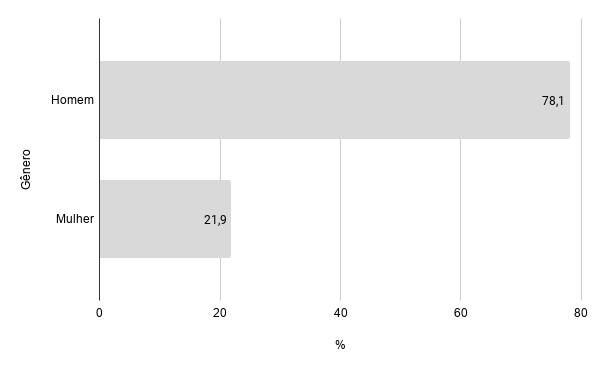
\includegraphics[width=.70\textwidth]{images/s_genero.png}
        \label{figure:s_genero}
        \caption{Gênero.}
        \end{figure}
    
    
    %\item Figura \ref{figure:s_idade}: Idade.
        \begin{figure}[!htb]
        \centering
        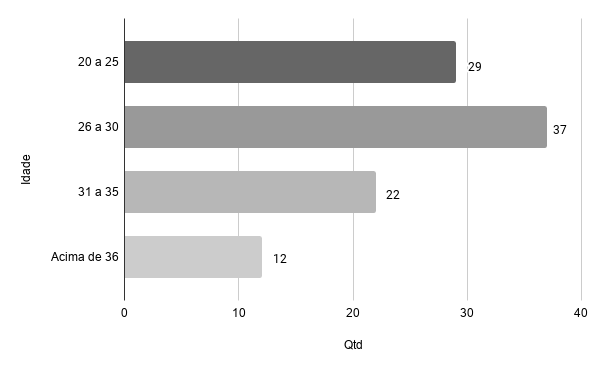
\includegraphics[width=.70\textwidth]{images/s_idade.png}
        \label{figure:s_idade}
        \caption{Idade.}
        \end{figure}
    
    
    %\item Figura \ref{figure:s_escolaridade}: Nível de escolaridade.
        \begin{figure}[!htb]
        \centering
        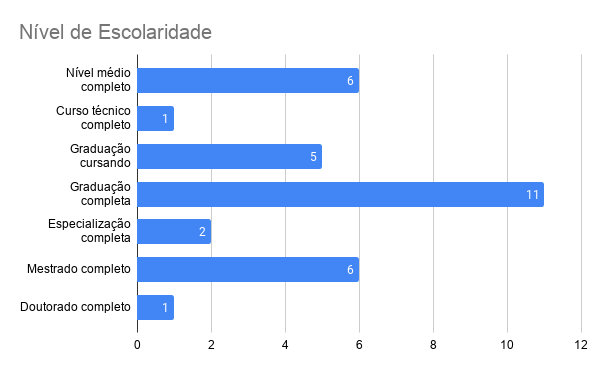
\includegraphics[width=.70\textwidth]{images/s_escolaridade.png}
        \label{figure:s_escolaridade}
        \caption{Nível de escolaridade.}
        \end{figure}
    
    
    %\item Figura \ref{figure:s_areaformacaoacademica}: Área de Formação Acadêmica.
        \begin{figure}[!htb]
        \centering
        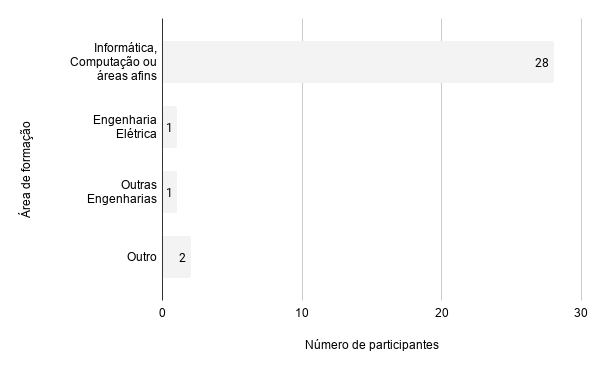
\includegraphics[width=.80\textwidth]{images/s_areaformacaoacademica.png}
        \label{figure:s_areaformacaoacademica}
        \caption{Área de formação acadêmica.}
        \end{figure}
    
    
    %\item Figura \ref{figure:s_certificacao}: Fez algum curso / certificação na área de testes?
        \begin{figure}[!htb]
        \centering
        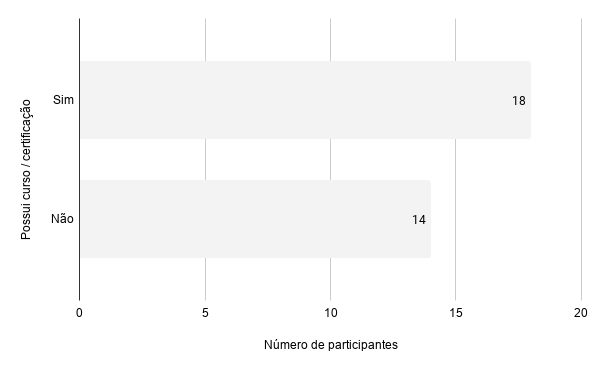
\includegraphics[width=.80\textwidth]{images/s_certificacao.png}
        \label{figure:s_certificacao}
        \caption{Você já fez algum curso / certificação na área de testes?}
        \end{figure}
    
    
    %\item Figura \ref{figure:s_certificacaodesc}: Caso a pergunta acima tenha sido "Sim", quais foram esses cursos / certificações?
        \begin{figure}[!htb]
        \centering
        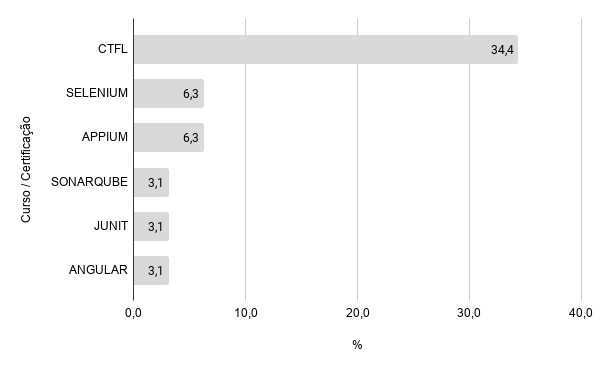
\includegraphics[width=.80\textwidth]{images/s_certificacaodesc.png}
        \label{figure:s_certificacaodesc}
        \caption{Caso a pergunta acima tenha sido "Sim", quais foram esses cursos / certificações?}
        \end{figure}
    
    
    %\item Figura \ref{figure:s_projetos}: Em relação a testes de projetos de apps Android, você:
        \begin{figure}[!htb]
        \centering
        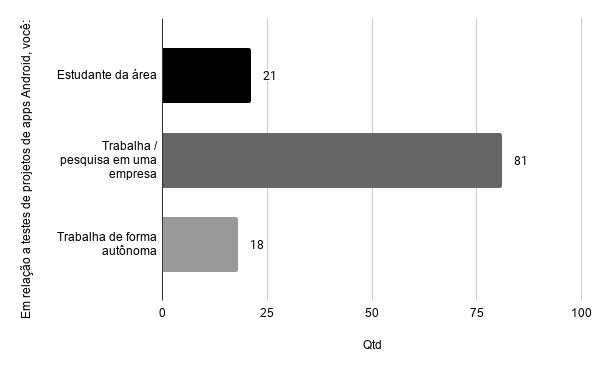
\includegraphics[width=.80\textwidth]{images/s_projetos.png}
        \label{figure:s_projetos}
        \caption{Em relação a testes de projetos de apps Android, você:}
        \end{figure}
    
    
    %\item Figura \ref{figure:s_estado}: Estado onde trabalha / estuda:
        \begin{figure}[!htb]
        \centering
        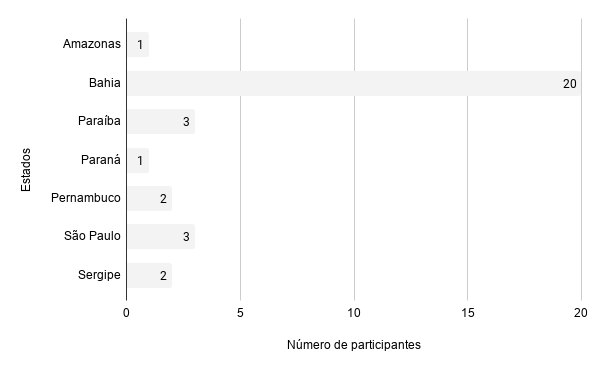
\includegraphics[width=.80\textwidth]{images/s_estado.png}
        \label{figure:s_estado}
        \caption{Estado onde trabalha / estuda:}
        \end{figure}


    %\item Figura \ref{figure:s_experienciatestes}: Experiência profissional na área de TESTES DE SOFTWARE:
        \begin{figure}[!htb]
        \centering
        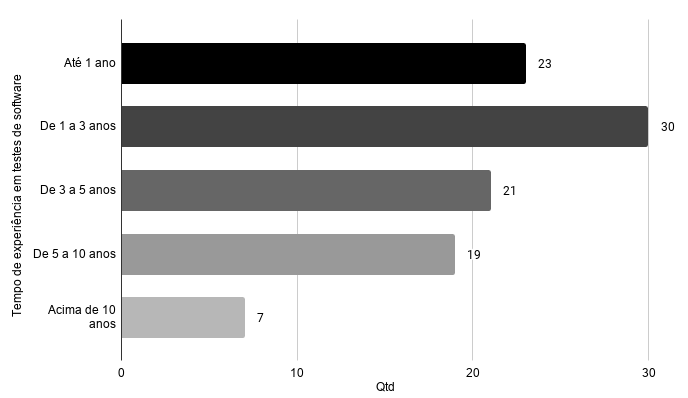
\includegraphics[width=.80\textwidth]{images/s_experienciatestes.png}
        \label{figure:s_experienciatestes}
        \caption{Experiência profissional na área de TESTES DE SOFTWARE:}
        \end{figure}
    

    %\item Figura \ref{figure:s_experienciatestesandroid}: Experiência profissional na área específica de TESTES DE APPS ANDROID:
        \begin{figure}[!htb]
        \centering
        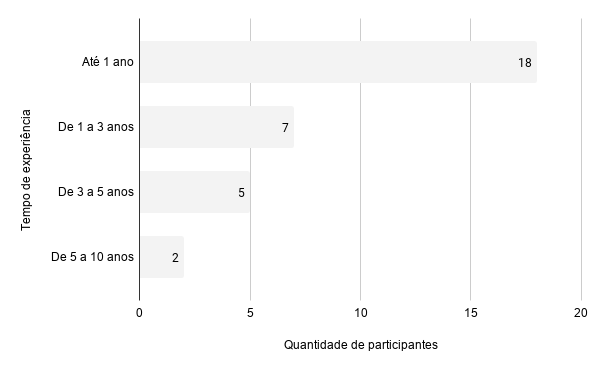
\includegraphics[width=.80\textwidth]{images/s_experienciatestesandroid.png}
        \label{figure:s_experienciatestesandroid}
        \caption{Experiência profissional na área específica de TESTES DE APPS ANDROID:}
        \end{figure}
    
    
     %\item Figura \ref{figure:s_conhecimentotestesandroid}: Quando comparado a outros profissionais, como você considera o seu nível de conhecimento em TESTES DE APPS ANDROID?
        \begin{figure}[!htb]
        \centering
        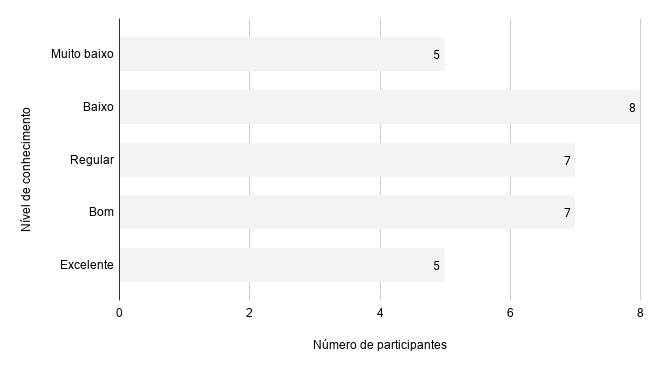
\includegraphics[width=.80\textwidth]{images/s_conhecimentotestesandroid.png}
        \label{figure:s_conhecimentotestesandroid}
        \caption{Quando comparado a outros profissionais, como você considera o seu nível de conhecimento em TESTES DE APPS ANDROID?}
        \end{figure}   
    
    
    \begin{comment}
        %\item Figura \ref{figure:s_funcaoprojeto}: Caso seja funcionário de uma empresa, qual a sua principal função no projeto atual?
        \begin{figure}[!htb]
        \centering
        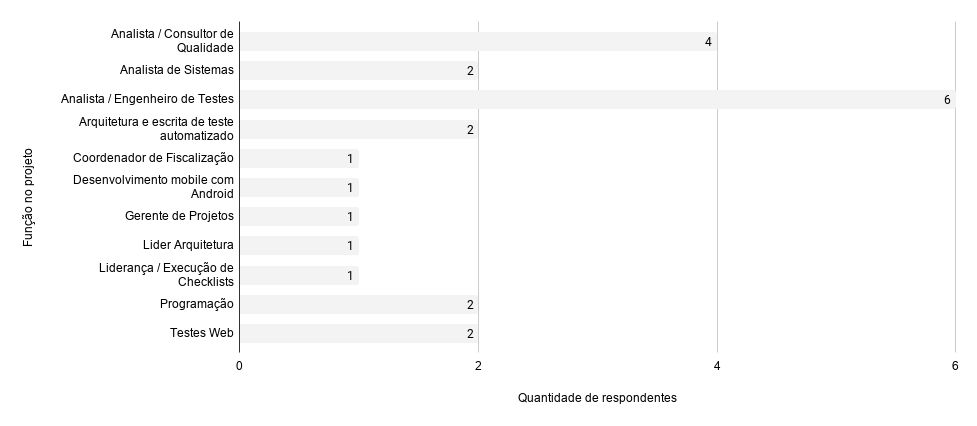
\includegraphics[width=.90\textwidth]{images/s_funcaoprojeto.png}
        \label{figure:s_funcaoprojeto}
        \caption{Caso seja funcionário de uma empresa, qual a sua principal função no projeto atual?}
        \end{figure}
    \end{comment}

    
    
    %\item Figura \ref{figure:s_atividadesprojeto}: Qual(is) atividade(s) realiza no processo de teste de software:
        \begin{figure}[!htb]
        \centering
        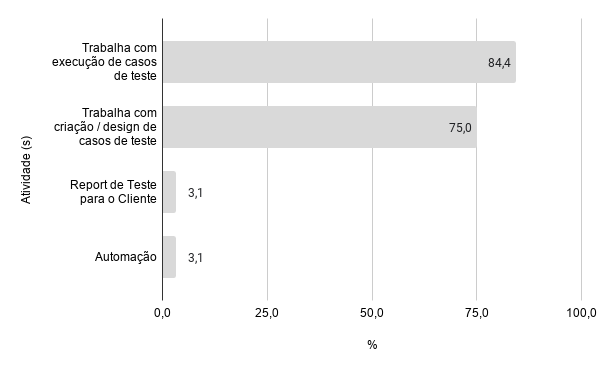
\includegraphics[width=.80\textwidth]{images/s_atividadesprojeto.png}
        \label{figure:s_atividadesprojeto}
        \caption{Qual(is) atividade(s) realiza no processo de teste de software:}
            \end{figure}   
    
    
    %\item Figura \ref{figure:s_categoriastestes}: Os testes realizados se enquadram em qual(is) categorias:
        \begin{figure}[!htb]
        \centering
        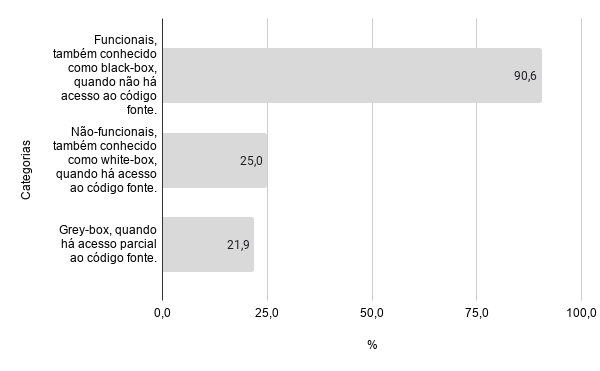
\includegraphics[width=.80\textwidth]{images/s_categoriastestes.png}
        \label{figure:s_categoriastestes}
        \caption{Os testes realizados se enquadram em qual(is) categorias:}
        \end{figure}       
    
  
     %\item Figura \ref{figure:s_tipostestes}: Qual(is) tipo(s) de teste são feitos:
        \begin{figure}[!htb]
        \centering
        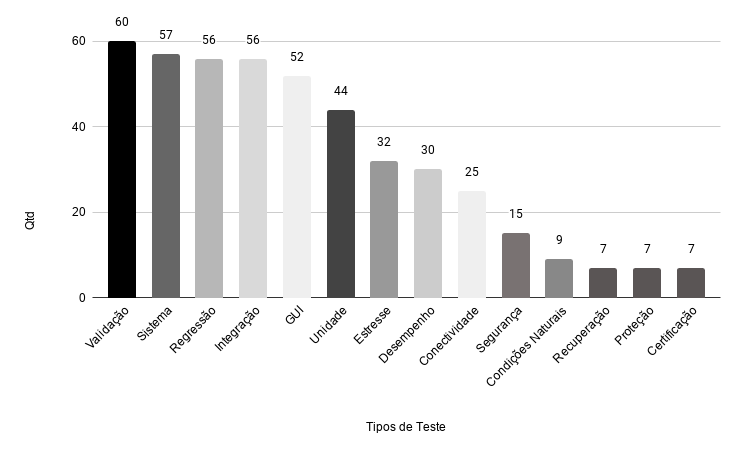
\includegraphics[width=.90\textwidth]{images/s_tipostestes.png}
        \label{figure:s_tipostestes}
        \caption{Qual(is) tipo(s) de teste são feitos:}
        \end{figure}
    
    
     %\item Figura \ref{figure:s_formatestes}: Os testes são realizados de forma:
        \begin{figure}[!htb]
        \centering
        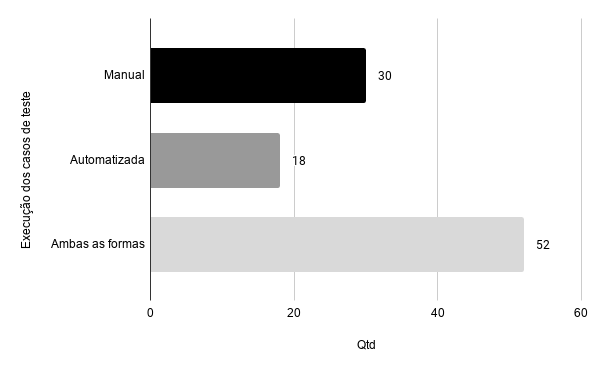
\includegraphics[width=.80\textwidth]{images/s_formatestes.png}
        \label{figure:s_formatestes}
        \caption{Os testes são realizados de forma:}
        \end{figure}    
    
    
    %\item Figura \ref{figure:s_ferramentastestes}: Quais ferramentas você costuma utilizar em seus projetos de APPS ANDROID?
        \begin{figure}[!htb]
        \centering
        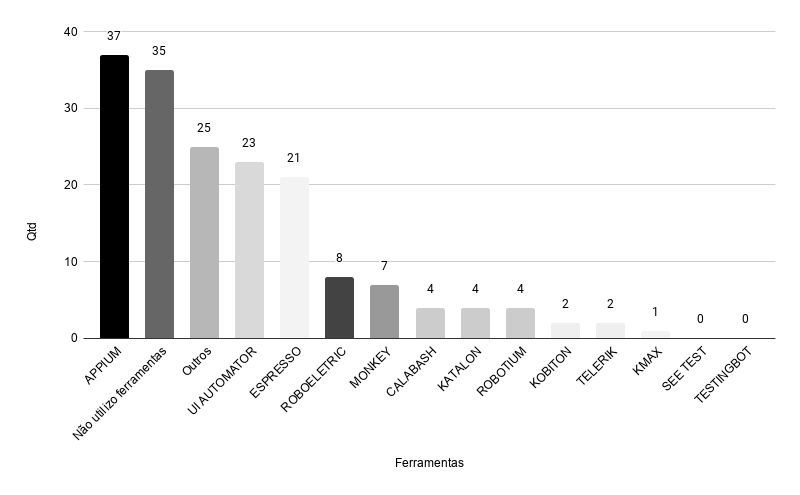
\includegraphics[width=.80\textwidth]{images/s_ferramentastestes.png}
        \label{figure:s_ferramentastestes}
        \caption{Quais ferramentas você costuma utilizar em seus projetos de APPS ANDROID?}
        \end{figure}
    
    
    %\item Figura \ref{figure:s_testemanutencao}: Quando é realizada uma MANUTENÇÃO (ATUALIZAÇÃO) no app Android, quer seja perfectiva, corretiva, adaptativa ou preventiva, é realizado algum tipo de teste com o objetivo de garantir que as manutenções realizadas não alteraram o comportamento funcional do app?
        \begin{figure}[!htb]
        \centering
        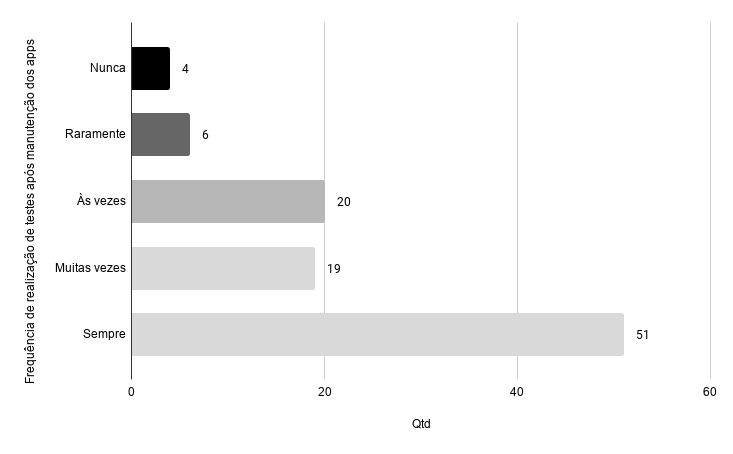
\includegraphics[width=.80\textwidth]{images/s_testemanutencao.png}
        \label{figure:s_testemanutencao}
        \caption{Quando é realizada uma MANUTENÇÃO (ATUALIZAÇÃO) no app Android, quer seja perfectiva, corretiva, adaptativa ou preventiva, é realizado algum tipo de teste com o objetivo de garantir que as manutenções realizadas não alteraram o comportamento funcional do app?}
        \end{figure}   
    
    
    %\item Figura \ref{figure:s_formatestemanutencao}: Caso, a resposta anterior seja positiva, o processo de teste durante MANUTENÇÃO (ATUALIZAÇÃO) do app é feita de que forma?
        \begin{figure}[!htb]
        \centering
        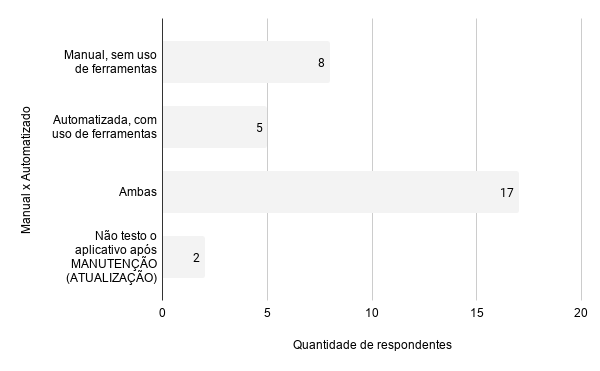
\includegraphics[width=.80\textwidth]{images/s_formatestemanutencao.png}
        \label{figure:s_formatestemanutencao}
        \caption{Caso, a resposta anterior seja positiva, o processo de teste durante MANUTENÇÃO (ATUALIZAÇÃO) do app é feita de que forma?}
        \end{figure}     
    
    
    %\item Figura \ref{figure:s_processostestemanutencao}: Quais processos você realiza para testar a versão atualizada do app:
        \begin{figure}[!htb]
        \centering
        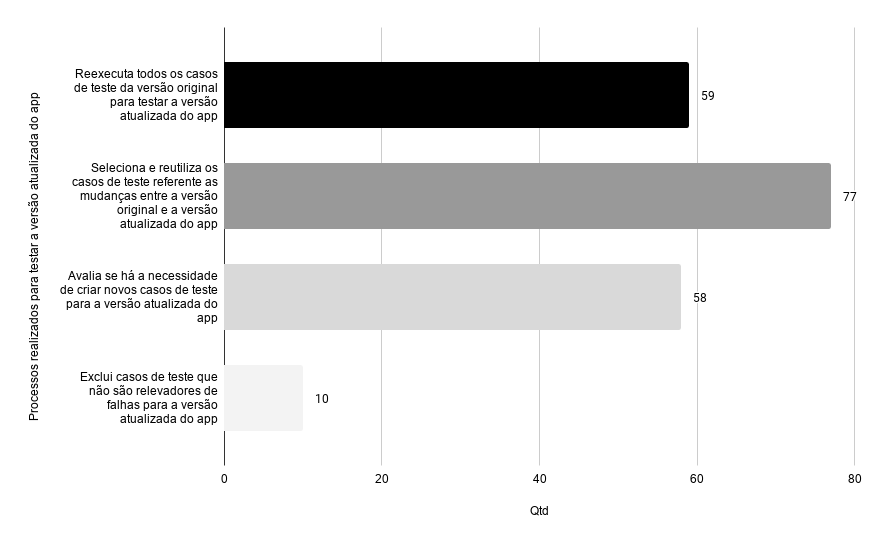
\includegraphics[width=.80\textwidth]{images/s_processostestemanutencao.png}
        \label{figure:s_processostestemanutencao}
        \caption{Quais processos você realiza para testar a versão atualizada do app:}
        \end{figure} 
    
    
    %\item Figura \ref{figure:s_testenovo}: Quando realiza alguma MANUTENÇÃO (ATUALIZAÇÃO) utiliza alguma ferramenta para automatizar o teste da nova versão do APP ANDROID?
        \begin{figure}[!htb]
        \centering
        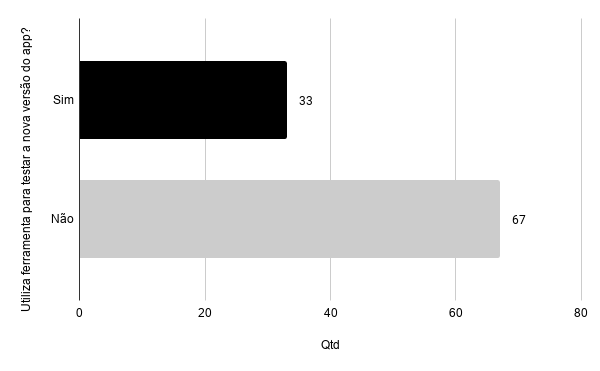
\includegraphics[width=.80\textwidth]{images/s_testenovo.png}
        \label{figure:s_testenovo}
        \caption{Quando realiza alguma MANUTENÇÃO (ATUALIZAÇÃO) utiliza alguma ferramenta para automatizar o teste da nova versão do APP ANDROID?}
        \end{figure}
    
    
    %\item Figura \ref{figure:s_ferramentastestenovo}: Caso utilize, qual(is) são a(s) ferramenta(s)?
        \begin{figure}[!htb]
        \centering
        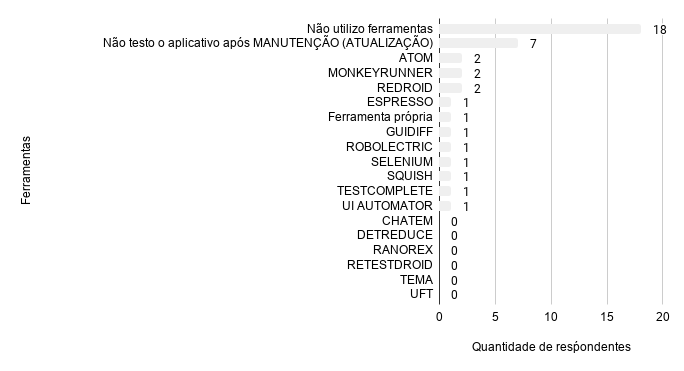
\includegraphics[width=.80\textwidth]{images/s_ferramentastestenovo.png}
        \label{figure:s_ferramentastestenovo}
        \caption{Caso utilize, qual(is) são a(s) ferramenta(s)?}
        \end{figure}
    
    
    %\item Figura \ref{figure:s_ferramentasexpectativas}: A(s) ferramenta(s) utilizada(s) atendem as necessidades para testar o app após ATUALIZAÇÃO (MANUTENÇÃO)?
        \begin{figure}[!htb]
        \centering
        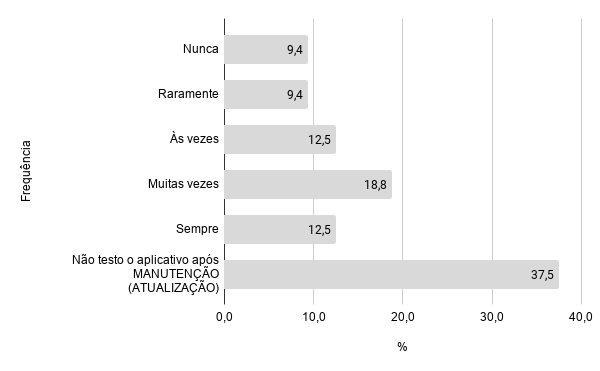
\includegraphics[width=.80\textwidth]{images/s_ferramentasexpectativas.png}
        \label{figure:s_ferramentasexpectativas}
        \caption{A(s) ferramenta(s) utilizada(s) atendem as necessidades para testar o app após ATUALIZAÇÃO (MANUTENÇÃO)?}
        \end{figure}
    
    \begin{comment}
    %\item Figura \ref{figure:s_jferramentasexpectativas}: Justifique a resposta anterior:
        \begin{figure}[!htb]
        \centering
        \includegraphics[width=.80\textwidth]{images/s_jferramentasexpectativas.png}
        \label{figure:s_jferramentasexpectativas}
        \caption{Justifique a resposta anterior:}
        \end{figure}
    \end{comment}
    
    
    %\item Figura \ref{figure:s_imptestarmanutencao}: Considera relevante testar apps ao realizar algum tipo de MANUTENÇÃO (ATUALIZAÇÃO)?
        \begin{figure}[!htb]
        \centering
        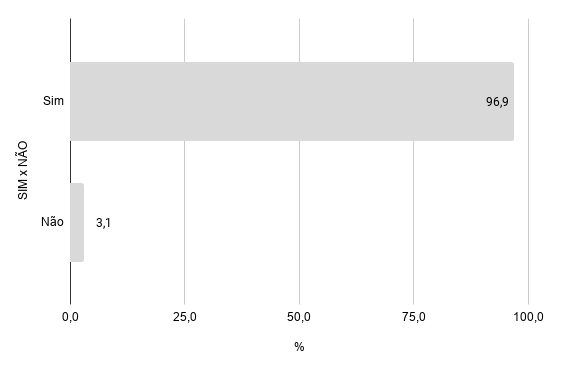
\includegraphics[width=.80\textwidth]{images/s_imptestarmanutencao.png}
        \label{figure:s_imptestarmanutencao}
        \caption{Considera relevante testar apps ao realizar algum tipo de MANUTENÇÃO (ATUALIZAÇÃO)?}
        \end{figure}
    
    
    %\item Figura \ref{figure:s_fatorestestemanutencao}: Qual(is) fator(es) você considera que fazem com que não sejam feitos testes em aplicativos após realização de MANUTENÇÃO (ATUALIZAÇÃO):
        \begin{figure}[!htb]
        \centering
        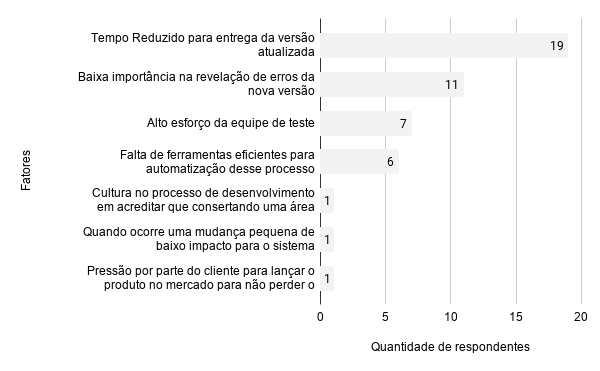
\includegraphics[width=.80\textwidth]{images/s_fatorestestemanutencao.png}
        \label{figure:s_fatorestestemanutencao}
        \caption{Qual(is) fator(es) você considera que fazem com que não sejam feitos testes em aplicativos após realização de MANUTENÇÃO (ATUALIZAÇÃO):}
        \end{figure}
    
   \begin{comment}
     % \item Figura \ref{figure:s_featuresfmanutencao}: Na sua opinião, quais são as features / funcionalidades que as ferramentas de teste precisam implementar para melhorar / automatizar o processo de testes  durante a manutenção de apps Android? Justifique sua resposta.
        \begin{figure}[!htb]
        \centering
        \includegraphics[width=.80\textwidth]{images/featuresfmanutencao.png}
        \label{figure:s_featuresfmanutencao}
   %    \caption{Na sua opinião, quais são as features / funcionalidades que as ferramentas de teste precisam implementar para melhorar / automatizar o processo de testes  durante a manutenção de apps Android? Justifique sua resposta.}
        \end{figure} 
   \end{comment}
   
    
    
    %\item Figura \ref{figure:s_featuresexistentes}: Você está satisfeito(a) com as features  / funcionalidades oferecidas pelas ferramentas de testes de app Android existentes?
        \begin{figure}[!htb]
        \centering
        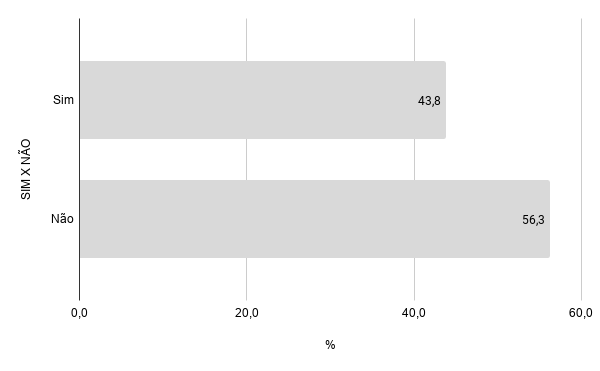
\includegraphics[width=.80\textwidth]{images/s_featuresexistentes.png}
        \label{figure:s_featuresexistentes}
        \caption{Você está satisfeito(a) com as features  / funcionalidades oferecidas pelas ferramentas de testes de app Android existentes?}
        \end{figure}

\begin{comment}
      % \item Figura \ref{figure:s_jfeaturesexistentes}: Justifique a sua resposta:
    \begin{figure}[!htb]
    \centering
    \includegraphics[width=.80\textwidth]{images/s_jfeaturesexistentes.png}
   \label{figure:s_jfeaturesexistentes}
   \caption{Justifique a sua resposta:}
   \end{figure}   
\end{comment}

    
    
%\end{itemize}


















\end{document}




